\documentclass[final]{cas-dc}

% ===== packages =====
\usepackage[utf8]{inputenc}
\usepackage{helvet}
\usepackage[round]{natbib}
\usepackage{amsmath,amssymb}
\usepackage{graphicx}
\usepackage{tikz}
\usetikzlibrary{positioning,arrows.meta,calc,shapes.geometric,backgrounds,fit}
\usepackage{booktabs}
\usepackage{array}
\usepackage{tabularx}
\usepackage{xcolor}
\usepackage{enumitem}
\usepackage{placeins}

% ===== light styling =====
\definecolor{legalblue}{RGB}{20,60,120}
\definecolor{citeblue}{RGB}{0,102,204}
\setlist{nosep, leftmargin=*}
\renewcommand{\arraystretch}{1.2}
\hypersetup{colorlinks=true, linkcolor=citeblue, citecolor=citeblue, urlcolor=citeblue,
  pdfborder={0 0 0}, breaklinks=true}

% ===== float tuning =====
\setcounter{topnumber}{3}
\setcounter{totalnumber}{5}
\renewcommand{\topfraction}{0.95}
\renewcommand{\bottomfraction}{0.9}
\renewcommand{\textfraction}{0.05}
\renewcommand{\floatpagefraction}{0.8}

\begin{document}

\ExplSyntaxOn
\RenewDocumentCommand \printorcid { }
{
  \seq_if_empty:NF \g_stm_orcid_seq
  {
    \group_begin:
      \tex_let:D \thefootnote \relax \footnotetext
      {
        \raggedright
        \textsc{orcid}(s):\c_space_token
        \seq_use:Nn \g_stm_orcid_seq { ;~ }
      }
    \group_end:
  }
}
\ExplSyntaxOff

\shortauthors{Hamza}
\shorttitle{Legal AI: From Case-Based Reasoning to Structure-Aware RAG}

\title[weight=\bfseries, size=\Huge]{Legal Artificial Intelligence: From Case-Based Reasoning to Reliable, Structure-Aware Retrieval-Augmented Generation}

\author{Ali Hamza}
\cormark[1]
\ead{ahamza.msse25mcs@student.nust.edu.pk}

\author{Imran Usman}

\author{Rabia Khan}

\affiliation{organization={National University of Sciences and Technology (NUST)},
            city={Islamabad},
            country={Pakistan}}

\cortext[1]{Corresponding author.}

\begin{abstract}
Legal work depends on finding, interpreting, and applying authoritative texts, such as statutes,
regulations, prior decisions, and procedural rules. A useful legal AI system must connect every
claim to a reliable legal source, not just produce fluent language. This survey presents the
development of legal artificial intelligence as one chronological journey, beginning with Ashley's
case-based reasoning system HYPO in 1991 and ending with Legalyze in 2026. We introduce each stage
in the order it was published, moving from early reasoning and prediction through domain-adapted
language models to retrieval-augmented generation and contemporary benchmarks. Legalyze and the
data-synthesis approach of Ren et al.\ (2026) serve as a comparative case study of two
complementary design philosophies. We bring this account together through three synthesis
chapters, covering reliability and citation verification, jurisdictional and multilingual access
with attention to Pakistan, and open research challenges. Throughout, we restrict every claim to
literature we could independently verify.
\end{abstract}

\begin{keywords}
Legal artificial intelligence \sep Retrieval-augmented generation \sep Legal information retrieval \sep Legal language models \sep Structure-aware retrieval \sep Hallucination \sep Citation verification \sep Pakistani legal AI
\end{keywords}

\maketitle

\section{Introduction}
\label{sec:intro}

A legal answer is only as good as the authority behind it. An explanation that reads smoothly but
cites the wrong statute, overlooks a controlling precedent, or misses a recent amendment is not a
minor flaw; it is a wrong answer, and one with real consequences for whoever relies on it. This is
what sets legal information systems apart from general-purpose question answering. A useful legal
system must identify the statutes and precedents that actually govern a question, interpret them in
the context that gives them meaning, show how they relate to one another, and present conclusions a
reader can check against the original source. Exact statutory wording matters. A provision's
relationship to its subordinate clauses matters. The authority of a judicial decision matters, and
so do the jurisdiction and date a rule applies to. A response can get any one of these wrong while
still sounding confident and complete, which is precisely what makes legal retrieval harder than
most other retrieval problems. Building a system that respects all of these constraints at once has
occupied legal AI research for more than three decades, and the problem is still open today.

This survey tells that three-decade story as a single, continuous narrative, in the order it
actually happened. Legal artificial intelligence (legal AI) did not arrive through one breakthrough;
it grew through a long sequence of smaller advances, each responding to a specific limitation in the
work before it. The story begins in 1991, when Kevin Ashley's case-based reasoning system HYPO showed
that a computer could compare a new legal dispute with earlier cases and identify the similarities
and differences that make a legal argument \citep{ashley1991}. We take HYPO as our starting point and
move forward year by year, introducing every system, benchmark, and finding in the order the field
actually published it. A reader who wants to understand how today's legal retrieval-augmented
generation (RAG) systems came to exist should be able to retrace the same path the field itself took,
without jumping between decades or topics. So the structure of this survey is the timeline of the
field itself, not a set of themes we arranged for convenience.

Three questions recur across this history, and they give the survey its structure. First,
\emph{how should legal knowledge be represented?} Early systems encoded it as explicit rules and
case comparisons; later systems learned it as patterns in text; the most recent systems treat it as
an external, inspectable corpus that a model retrieves from rather than memorizes. Second, \emph{how
should relevant legal evidence be found?} The field moved from simple keyword matching, to semantic
and hybrid retrieval, to retrieval that tries to preserve the hierarchical structure of a statute or
the reasoning inside a judgment. Third, \emph{how should a system's answer be trusted?} Once
language models became fluent enough to sound authoritative whether or not they were right, the
field had to build ways of checking a generated claim against the evidence that is meant to support
it. These three questions, representation, retrieval, and trust, organize everything that follows.

This survey makes four contributions. First, a \textbf{chronological synthesis} that traces legal
AI's development in the exact order it happened, from case-based reasoning to contemporary
structure-aware retrieval-augmented generation, explaining the problem that motivated each new piece
of work. Second, an \textbf{architectural analysis} that separates document representation,
retrieval, rank fusion, generation, and evidence verification in the order the field introduced
them, and shows how each component feeds into overall reliability. Third, a \textbf{focused
comparative case study} of two systems published in 2026, Legalyze and the data-synthesis approach
of Ren et al., which target different parts of the same pipeline. Fourth, a \textbf{research agenda}
covering open challenges in structure-preserving retrieval, jurisdiction-aware evidence selection,
multilingual legal access, and verifiable answer generation. Table~\ref{tab:rq} summarizes the
research questions behind these four contributions.

\begin{table*}[t]
\centering
\caption{Research questions guiding the survey.}
\label{tab:rq}
\footnotesize
\setlength{\tabcolsep}{5pt}
\renewcommand{\arraystretch}{1.25}
\begin{tabularx}{\textwidth}{>{\raggedright\arraybackslash}X >{\raggedright\arraybackslash}X}
\toprule
\textbf{Research question} & \textbf{Purpose} \\
\midrule
\textbf{RQ1.} How did legal AI evolve, in the order it actually happened, from case-based reasoning to RAG? & Present the principal methodological transitions and the limitations that motivated each one, in sequence. \\
\textbf{RQ2.} How do legal retrieval architectures affect evidence quality? & Explain how systems locate relevant authorities and preserve the context needed to interpret them. \\
\textbf{RQ3.} How should we assess reliability in legal AI? & Distinguish fluent generation from evidence-supported legal answers. \\
\textbf{RQ4.} What challenges remain for jurisdiction-aware and multilingual legal AI? & Identify research opportunities across different legal and linguistic contexts. \\
\bottomrule
\end{tabularx}
\end{table*}

Section~\ref{sec:method} explains how we found, checked, and selected the literature for this
chronological account. The narrative itself then begins in Section~\ref{sec:foundations} with
Ashley's 1991 work on HYPO.

\section{Review Methodology}
\label{sec:method}

This study uses a structured, chronological narrative review of legal artificial intelligence.
Instead of grouping the literature by topic, it follows the order of publication. Each advance
appears after the work that motivated it and before the work that responded to it. This design
suits a field that spans several related but distinct areas. These include legal knowledge
representation, natural language processing, information retrieval, large language models, and
evidence verification. The design also matches the review's purpose directly. We want to explain how
each change in system design responded to a limitation of what came before it, not to rank models by
a single reported score.

We identified relevant literature across computer science and legal informatics sources, including
Scopus, Web of Science, IEEE Xplore, the ACM Digital Library, the ACL Anthology, Google Scholar,
official publisher and proceedings pages, and arXiv. The search combined four term groups: the legal
domain (for example, ``legal AI'' or ``case-based reasoning''), the underlying technology (``legal
language model'', ``LEGAL-BERT''), retrieval and document structure (``hybrid retrieval'',
``structure-aware indexing'', ``knowledge graph''), and reliability (``legal hallucination'',
``citation verification''). We supplemented keyword search with backward and forward citation
searching to catch studies that different terminology might have hidden. Table~\ref{tab:sel}
summarizes the selection criteria we applied to the resulting records.

\begin{table*}[t]
\centering
\caption{Study selection criteria.}
\label{tab:sel}
\footnotesize
\setlength{\tabcolsep}{5pt}
\renewcommand{\arraystretch}{1.25}
\begin{tabularx}{\textwidth}{>{\raggedright\arraybackslash}p{2.6cm} >{\raggedright\arraybackslash}X >{\raggedright\arraybackslash}X}
\toprule
\textbf{Criterion} & \textbf{Include} & \textbf{Exclude} \\
\midrule
Topical relevance & Legal reasoning, legal NLP, retrieval, generation, verification, or evaluation. & AI in an unrelated domain with no meaningful link to legal information processing. \\
Technical contribution & A method, architecture, dataset, benchmark, or substantive empirical finding. & Mentions legal AI only in passing, with no relevant technical content. \\
Venue quality & A peer-reviewed article or proceedings paper in an established, well-indexed venue (a Q1-ranked journal or a recognized conference); foundational works; preprints that add substantial, clearly identified value. & Venues with no established standing in computer science or legal informatics, and non-scholarly material used as if it were primary research. \\
Evidence availability & An accessible bibliographic record, checked against the publisher's page or official proceedings, with a verifiable DOI where one exists. & Claims or publication details that cannot be independently verified. \\
Jurisdiction and language & Any jurisdiction or language relevant to the review's research questions. & No jurisdiction or language excluded solely for being under-represented. \\
\bottomrule
\end{tabularx}
\end{table*}

We included a record only after checking its bibliographic details against the publisher's page,
the official proceedings, or another authoritative source, and after verifying its DOI where one
exists. For preprints, we treated the consulted version as distinct from any later published
version. We checked venue quality deliberately. This survey keeps to Q1-ranked journals and
recognized conference venues, and we dropped a number of candidate papers at this stage because we
could not confirm their venue met that bar. For each included study, we recorded its research
objective, legal domain and jurisdiction, technical approach, evidence sources, evaluation method,
and acknowledged limitations. We then sorted this information into the thematic categories the
following sections use: historical foundations, legal language models, retrieval architecture,
document and knowledge representation, generation and orchestration, reliability and verification,
and evaluation design.

We present the resulting set of studies in original publication order, year by year, instead of
grouping them by theme. This lets the historical account in Section~\ref{sec:foundations} and onward read as one
continuous development rather than a set of separately ordered topics. We report quantitative
results only together with their original experimental context, because studies differ in
jurisdiction, corpus, query set, and definition of success. A legal classification benchmark, for
instance, cannot be compared directly with a human evaluation of unsupported legal claims. Throughout
the survey we keep three kinds of statements separate: findings individual studies report directly,
interpretations we draw by comparing multiple studies, and open questions for future research. That
discipline, together with our restriction to independently verifiable, well-indexed sources, keeps
this a critical narrative of the field rather than a catalogue of publications.

\section{Foundations: Case-Based Reasoning and Rule-Based Systems (1991--2009)}
\label{sec:foundations}

Figure~\ref{fig:landscape} previews the full journey this survey takes, from 1991 to 2026, as a
conceptual orientation device only. The narrative below, and every section that follows, cites the
specific, independently verifiable study behind each stage, and we cite these studies in the exact
order the field published them, so that the figure and the citation record agree with each other.

\begin{figure*}[tp]
\centering
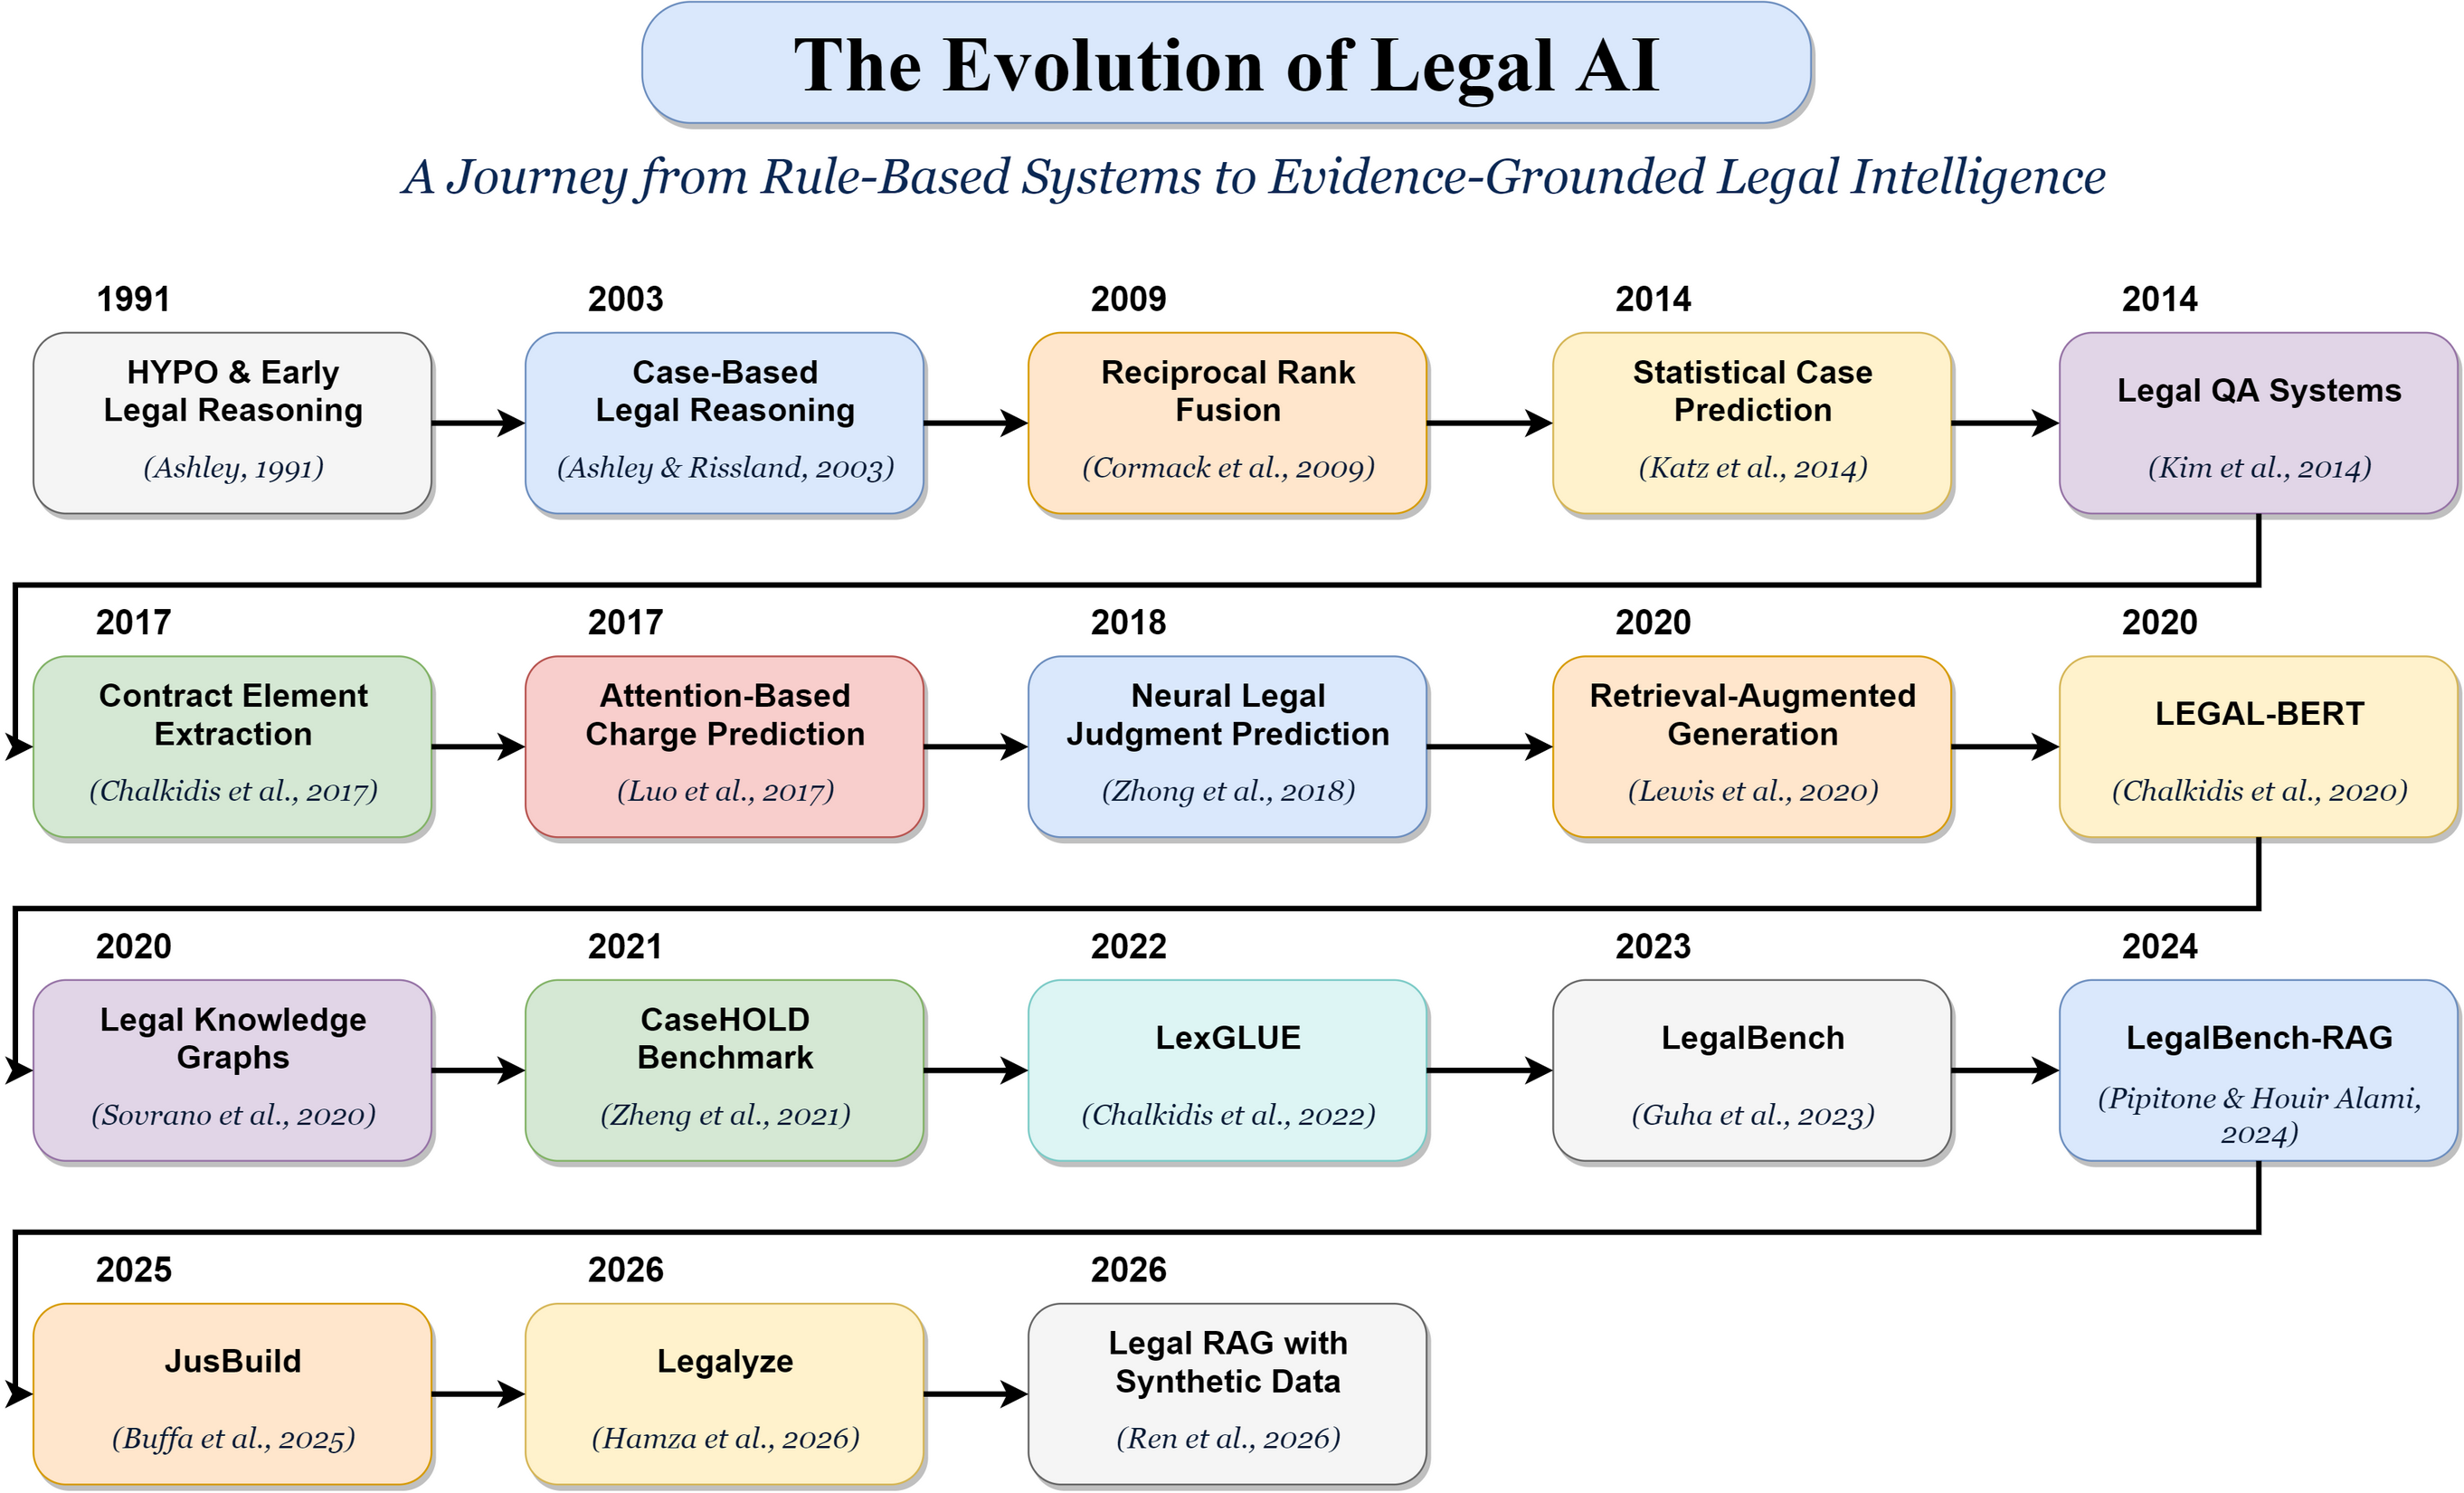
\includegraphics[width=\textwidth]{images/evolution_of_legal_ai.png}
\caption{The evolution of legal AI, 1991--2026, read as a sequence of methodological responses
rather than isolated dates: transparent but non-scaling reasoning systems (case-based reasoning,
rule-based expert systems); learned legal language representations and shared benchmarks; and
recent work on retrieval-augmented generation, reliability, and structure-aware retrieval. The
verified study underpinning each stage is cited, in chronological order, in
Sections~\ref{sec:foundations}--\ref{sec:2026}.}
\label{fig:landscape}
\end{figure*}

\subsection{1991: can a computer reason with cases?}

The field's starting question was foundational: can a computer represent the knowledge and
reasoning that legal professionals use to resolve disputes? Kevin Ashley's HYPO system, published in
1991, gave the first influential answer. HYPO compared a new fact pattern with earlier cases, picked
out the similarities and differences that matter legally, and built arguments from those comparisons
\citep{ashley1991}. This was a deliberate design choice: HYPO did not treat a past decision as a
ready-made answer to a new question, but instead made the comparison process itself part of the
computational problem. The system showed that legal relevance depends on more than textual
similarity between a query and a precedent; it depends on which facts a court would treat as
decisive.

A related line of work, running at the same time, built rule-based expert systems that represented
legal knowledge directly as explicit rules applied to known facts. This made their reasoning easy to
inspect, since a developer could trace exactly which rule and which condition produced a given
output, but it also made them expensive to maintain: legislation changes, exceptions pile up, and
different authorities apply in different circumstances, so a system's rules have to be updated by
hand to keep pace. Structured knowledge representation, including legal ontologies, offered a
complementary response by defining legal concepts and the relationships between them explicitly.
Much later, this idea matured into the knowledge-graph-based legal retrieval systems we discuss in
Section~\ref{sec:lm2023}.

\subsection{2003: case-based reasoning as a form of learning}

Twelve years after HYPO, Ashley and Rissland gave a more general account of why this style of
reasoning works. In \emph{Law, Learning and Representation}, they framed case-based legal reasoning
as a form of \emph{lazy learning}: a court, on this view, holds off generalizing from past cases
until it knows the facts of the new case, rather than committing in advance to one fixed rule
\citep{ashley2003}. This reframing tied case-based reasoning explicitly to machine learning and to
legal information retrieval, and it also clarified what the foundational period had actually
established: a legal AI system needs both a representation of legal knowledge and a method for
applying that representation to the specific facts of a new dispute. A system may have explicit
rules and still fail to identify which facts matter, or it may retrieve a similar case and still
fail to explain why the differences between it and the new dispute matter. That distinction still
organizes legal AI research today.

Alongside reasoning about cases, this period raised a different but related question: how do you
simply \emph{find} the legal documents relevant to a user's need? Legal information retrieval is not
the same problem as legal reasoning; retrieval ranks potentially relevant material, while reasoning
determines how a reader should interpret and apply that material. Early retrieval work leaned
heavily on lexical evidence, which is useful in law because exact wording, section numbers, and
established legal phrases can be decisive, but it can miss material when a query and an
authoritative document describe the same legal concept in different words.

\subsection{2009: a general retrieval technique, outside the legal domain, that the field would later adopt}

The last foundational building block in this period did not come from legal AI at all. In 2009,
\citet{cormack2009} introduced Reciprocal Rank Fusion (RRF) at a general information-retrieval
venue, offering a simple way to combine several ranked lists of search results into one. RRF scores
a candidate document using the reciprocal of its rank in each contributing list,
\begin{equation}
\operatorname{RRF}(d)=\sum_{r \in R}\frac{1}{k+\operatorname{rank}_{r}(d)},
\end{equation}
where $d$ is a candidate document, $R$ is the set of ranked retrieval results under combination,
$\operatorname{rank}_r(d)$ is the rank of $d$ in list $r$, and $k$ is a smoothing constant. Its
appeal is that it combines rankings without needing the underlying retrieval methods to produce
directly comparable scores, which matters because two different retrieval methods often produce
scores on entirely different scales: one method might rely on exact wording, while another might
rely on semantic similarity. We introduce RRF here, at its true publication date, precisely because
it is general purpose; it carries no legal content of its own, and this survey will not pretend
otherwise. It resurfaces more than a decade later, in Section~\ref{sec:rag2024}, once legal retrieval
systems need to combine lexical and semantic evidence, and that is where its legal relevance
actually begins.

\subsection{What this period established}

By the end of this period, legal AI had built up complementary foundations rather than a single
architecture. Case-based reasoning showed that legal relevance requires comparing the facts of
disputes, not just their words. Rule-based systems and legal ontologies showed that legal AI could
represent legal knowledge explicitly, at the cost of ongoing maintenance as the law changes. Early
information retrieval showed that finding candidate legal material is a distinct problem from
reasoning about it. And outside the field entirely, general-purpose information retrieval was
developing techniques, such as rank fusion, that legal AI would not need until its own retrieval
systems grew more sophisticated. None of these approaches alone solved the full challenge of finding
authoritative evidence, keeping its context, and producing a reliable answer. The next advance in
the field's actual chronology did not arrive until 2014, when researchers began asking a different
question: not how should a system reason about a case, but could data alone predict a case's
outcome?

\section{Quantifying and Predicting Legal Outcomes (2014--2018)}
\label{sec:outcomes}

\subsection{2014: predicting a court's decision from data}

The next advance did not come from representing legal reasoning more carefully. It came from a
different question: could statistics predict a court's decision, with no explicit model of legal
reasoning at all? In 2014, \citet{katz2014} built a time-evolving statistical classifier, training it
on historical voting and case data to predict the outcomes of United States Supreme Court decisions.
Their method used an ensemble of decision trees, a random-forest classifier; it was not a language
model, and it was not a case-based comparison in Ashley's sense, but rather a quantitative
pattern-recognition problem over structured case features. The result mattered precisely because the
system did not need to represent legal rules or compare case facts the way HYPO did: it showed that
a purely statistical model, given enough historical data, could forecast judicial behavior with
useful accuracy. This also exposed a limitation that recurs throughout the rest of this survey. A
system can predict an outcome correctly while giving no account of the legal reasoning behind it,
which is a very different capability from explaining \emph{why} a court should decide a case a
particular way.

In the same year, a separate study took on a different question: not whether a system could predict
an outcome, but whether a system could answer a legal question directly. \citet{kim2014} built a
legal question-answering system that combines legal information retrieval with textual entailment,
ranking candidate answers with a support vector machine informed by syntactic and semantic
similarity. The authors evaluated it on the first Competition on Legal Information Extraction and
Entailment (COLIEE) dataset. Katz predicted an outcome from structured case data, while Kim retrieved
and compared legal text directly, and together they give a useful snapshot of 2014: the same year
produced an outcome-prediction system that bypassed legal text entirely, and a question-answering
system built entirely around retrieving and comparing it. The COLIEE benchmark this study helped
establish recurs throughout this survey, as later editions appear in subsequent years.

\subsection{2017: extracting structure from legal text, and predicting charges from facts}

Three years later, two separate lines of work, both published in 2017, pushed in a complementary
direction: instead of predicting an outcome from case metadata, they tried to connect a predicted
outcome back to the specific legal text that justifies it. \citet{chalkidis2017} took on contract
element extraction, applying neural sequence-labelling methods to identify defined terms,
obligations, and other structured elements directly within contract text. This was an early sign
that neural NLP methods could extract the kind of structured legal information earlier rule-based
systems had encoded by hand. In the same year, \citet{luo2017} proposed a model for predicting
criminal charges that explicitly retrieves and attends over the specific statutory articles that
justify a predicted charge. It uses an attention mechanism to connect the facts of a case to the law
articles it identifies as relevant, and the authors report that this explicit legal-basis signal
improved charge-prediction accuracy over models using case facts alone. Katz's 2014 model predicted
an outcome without reference to legal text, while Luo et al.'s model took a first step toward
grounding a predicted outcome in the specific statutory provisions that justify it. This anticipates
the evidence-grounding problem that motivates legal RAG later in this survey.

\subsection{2018: modelling legal judgment as several connected subtasks}

The following year, \citet{zhong2018} generalized this idea. Rather than predicting a single output,
a charge or a verdict, they observed that a real legal judgment involves several connected subtasks:
identifying the applicable law articles, determining the charge, and deciding the sentence term.
They modelled the dependencies among these subtasks as a directed acyclic graph and solved them
jointly through topological multi-task learning, reporting that representing these dependencies
explicitly improved performance over treating each subtask on its own. Compared with
\citet{katz2014} and \citet{luo2017}, this period teaches one specific and cumulative lesson: legal
judgment prediction benefits from representing the structure of a legal decision, not just its
textual facts. The rest of this survey shows the field relearning that lesson, in a different form,
as it moves from outcome prediction toward retrieval-augmented generation.

\subsection{What the foundational and prediction periods together established}

Table~\ref{tab:foundational} summarizes the approaches discussed so far, in the order the field
published them between 1991 and 2018.

\begin{table*}[tp]
\centering
\caption{Legal AI milestones discussed so far, in chronological order (1991--2018).}
\label{tab:foundational}
\footnotesize
\setlength{\tabcolsep}{5pt}
\renewcommand{\arraystretch}{1.25}
\begin{tabularx}{\textwidth}{>{\raggedright\arraybackslash}p{1.6cm} >{\raggedright\arraybackslash}p{2.9cm} >{\raggedright\arraybackslash}X >{\raggedright\arraybackslash}X}
\toprule
\textbf{Year} & \textbf{Study} & \textbf{Core idea} & \textbf{Principal limitation} \\
\midrule
1991 & \citet{ashley1991} (HYPO) & Compare a dispute with precedents and construct arguments from relevant similarities and differences. & Legally meaningful similarity, not textual similarity, must be identified. \\
2003 & \citet{ashley2003} & Reframe case-based legal reasoning as lazy, case-driven learning. & Does not by itself resolve how legal knowledge should be found or maintained at scale. \\
2009 & \citet{cormack2009} & Combine multiple ranked lists via Reciprocal Rank Fusion (general-purpose IR, not legal). & Carries no legal content; legal relevance only emerges once applied to legal retrieval, later in this survey. \\
2014 & \citet{katz2014} & Predict United States Supreme Court outcomes with a statistical, time-evolving classifier. & Predicts outcomes without explaining the applicable legal reasoning. \\
2014 & \citet{kim2014} & Answer legal questions by combining information retrieval with SVM-ranked textual entailment on COLIEE data. & Entailment between a question and a retrieved article, not broader legal reasoning. \\
2017 & \citet{chalkidis2017} & Extract structured elements (terms, obligations) from contracts with neural sequence labelling. & Extraction, not reasoning about the extracted elements. \\
2017 & \citet{luo2017} & Jointly predict criminal charges and the statutory articles that justify them. & Evaluated on Chinese criminal cases; generalization across jurisdictions untested. \\
2018 & \citet{zhong2018} & Model law article, charge, and sentence prediction as dependent subtasks solved jointly. & Predicts a judgment's components without retrieving or citing external authoritative sources. \\
\bottomrule
\end{tabularx}
\end{table*}

None of these approaches alone solved the problem of locating authoritative evidence, keeping its
context, and producing a legally justified answer. Together, though, they set up the two remaining
halves of the problem, and the rest of this survey follows them in order. The first half is
representing legal knowledge in a form a model can learn from, which the field pursued through
legal language models starting in 2020. The second half is retrieving external, verifiable evidence
instead of relying on what a model has memorized, which the field pursued through
retrieval-augmented generation starting in 2024. We take up the first of these next.

\section{Legal Language Models and Benchmarks (2020--2023)}
\label{sec:lm2023}

Two years after \citet{zhong2018}, the field's center of gravity shifted again. By 2020, large
pretrained language models had become capable enough that researchers could adapt a general-purpose
model to a new domain instead of building one from scratch for every task. This section follows how
the field first connected that capability to external evidence, then adapted it specifically to
legal text, then evaluated it systematically, all within a four-year window.

\subsection{2020: connecting generation to retrieved evidence, outside the legal domain}

The most consequential development of this period, for everything that follows in this survey, was
not legal at all when it first appeared. \citet{lewis2020} introduced retrieval-augmented generation
(RAG): instead of relying only on knowledge encoded in a model's parameters, a RAG system retrieves
external documents at inference time and conditions its generated output on them.
Figure~\ref{fig:lewis-rag} summarizes their architecture.

% The end-to-end retrieval-augmented generation (RAG) architecture of Lewis et al. (2020).
\begin{figure*}[t]
\centering
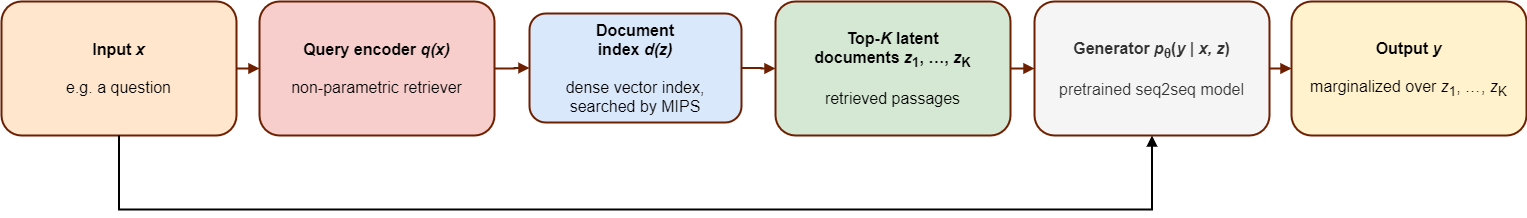
\includegraphics[width=\textwidth]{images/rag_original_architecture.png}
\caption{The end-to-end retrieval-augmented generation (RAG) architecture of
\citet{lewis2020}, redrawn here for discussion. A non-parametric retriever ($q(x)$ over a dense
document index $d(z)$, searched with Maximum Inner Product Search) returns the top-$K$ passages
for an input $x$; a parametric seq2seq generator then conditions on both $x$ and each retrieved
passage and the final output $y$ is marginalized over the retrieved set. This general-domain
architecture, not originally designed for law, is the direct ancestor of every legal RAG pipeline
discussed in the remainder of this survey.}
\label{fig:lewis-rag}
\end{figure*}


A non-parametric retriever, built from a query encoder and a dense document index searched with
Maximum Inner Product Search, returns the top-$K$ passages for an input, and a parametric seq2seq
generator then conditions on the input and each retrieved passage, with the final output
marginalizing over the retrieved set. Lewis et al.\ reported that this architecture improved
performance on knowledge-intensive, open-domain tasks, producing answers that were more specific and
better supported than generation from parameters alone. We introduce RAG here, at its true
publication date and in its original, general-purpose form, for the same reason we introduced
Reciprocal Rank Fusion in Section~\ref{sec:foundations}: researchers did not design it for law, and
this survey will not credit it as though they had. Its legal application came later, as a separate
development this survey reaches in Section~\ref{sec:rag2024}.

In the same year, two further developments addressed complementary problems. \citet{chalkidis2020}
introduced \textbf{LEGAL-BERT}, testing three strategies for adapting the BERT architecture to legal
text: using the original pretrained model as is, continuing its pretraining on legal corpora, or
pretraining a new model from scratch on legal text. They released a family of legal language models
for later research, illustrated in Figure~\ref{fig:legalbert}. The underlying principle is simple:
if a model has to process legal documents, its training should expose it to the language and
terminology those documents use. Readers should not treat LEGAL-BERT as a complete legal reasoning
system, though, since it provides learned language representations for specific NLP tasks; it does
not determine which authority governs a dispute, and it does not confirm that the cited text
supports a generated conclusion.

% Original diagram summarizing the three BERT adaptation strategies of Chalkidis et al.
% (2020), "LEGAL-BERT: The Muppets Straight out of Law School" (Findings of EMNLP 2020),
% Figure 1. Redrawn in this paper's own visual style; cited in the caption and surrounding text.
\begin{figure*}[t]
\centering
\resizebox{\textwidth}{!}{%
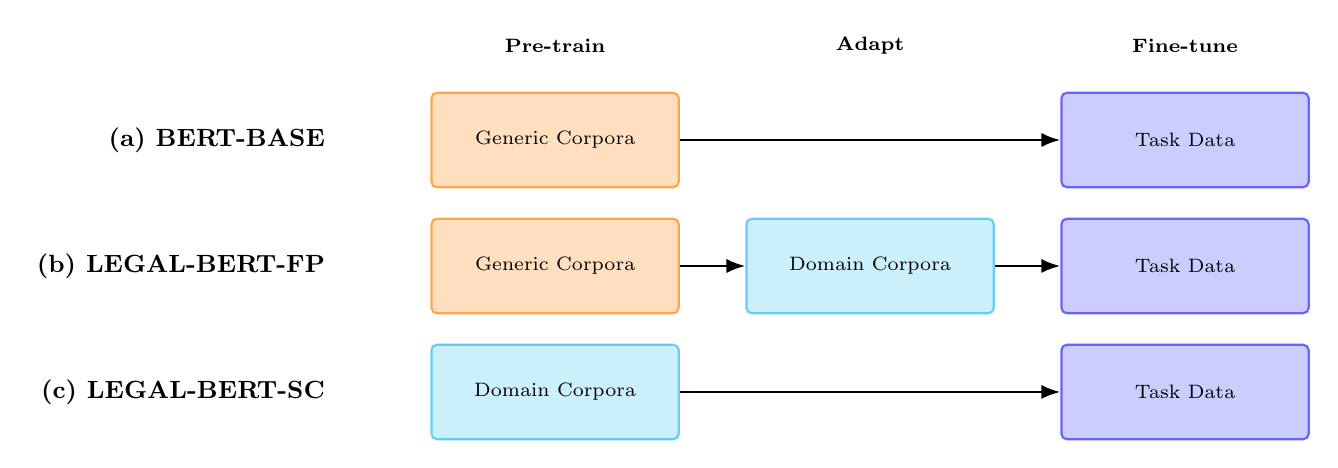
\begin{tikzpicture}[
  font=\scriptsize,
  lbl/.style={font=\scriptsize\bfseries, align=center},
  stg/.style={draw, thick, rounded corners=2pt, align=center, text width=3.0cm,
              minimum height=12mm, inner sep=2pt},
  rowlbl/.style={font=\small\bfseries, align=left, anchor=east}]

  \node[lbl] at (2.5,1.2)  {Pre-train};
  \node[lbl] at (6.5,1.2)  {Adapt};
  \node[lbl] at (10.5,1.2) {Fine-tune};

  % row (a) BERT-BASE
  \node[rowlbl] at (-0.3,0) {(a) BERT-BASE};
  \node[stg, fill=orange!25, draw=orange!70] (a1) at (2.5,0) {Generic Corpora};
  \node[stg, fill=blue!20, draw=blue!60]     (a3) at (10.5,0) {Task Data};
  \draw[-{Latex[length=2.4mm]}, line width=0.9pt] (a1) -- (a3);

  % row (b) LEGAL-BERT-FP
  \node[rowlbl] at (-0.3,-1.6) {(b) LEGAL-BERT-FP};
  \node[stg, fill=orange!25, draw=orange!70] (b1) at (2.5,-1.6) {Generic Corpora};
  \node[stg, fill=cyan!20, draw=cyan!60]     (b2) at (6.5,-1.6) {Domain Corpora};
  \node[stg, fill=blue!20, draw=blue!60]     (b3) at (10.5,-1.6) {Task Data};
  \draw[-{Latex[length=2.4mm]}, line width=0.9pt] (b1) -- (b2);
  \draw[-{Latex[length=2.4mm]}, line width=0.9pt] (b2) -- (b3);

  % row (c) LEGAL-BERT-SC
  \node[rowlbl] at (-0.3,-3.2) {(c) LEGAL-BERT-SC};
  \node[stg, fill=cyan!20, draw=cyan!60]     (c2) at (2.5,-3.2) {Domain Corpora};
  \node[stg, fill=blue!20, draw=blue!60]     (c3) at (10.5,-3.2) {Task Data};
  \draw[-{Latex[length=2.4mm]}, line width=0.9pt] (c2) -- (c3);

\end{tikzpicture}}
\caption{The three strategies for adapting BERT to a downstream legal NLP task, from
\citet{chalkidis2020}, redrawn here for discussion. (a) BERT-BASE uses the original pretrained
model as-is and fine-tunes directly on task data; (b) LEGAL-BERT-FP further pretrains BERT on
domain-specific (legal) corpora before fine-tuning; (c) LEGAL-BERT-SC pretrains a new model from
scratch on domain-specific corpora. All three alternatives share a final fine-tuning step on the
task data.}
\label{fig:legalbert}
\end{figure*}


Separately, \citet{sovrano2020} built legal knowledge graphs for question answering by combining
open knowledge-extraction tools with NLP techniques. This extended the structured-representation
idea legal ontologies first raised in Section~\ref{sec:foundations} into a form that could support
graph-based retrieval, a technique this survey returns to in Section~\ref{sec:rag2024}.

\subsection{2021: a harder benchmark for legal pretraining}

The following year, \citet{zheng2021} introduced \textbf{CaseHOLD}, a dataset built from the holding
statements of US case law. The authors designed it specifically to test whether domain-specific
pretraining measurably helps on a genuinely difficult legal task, identifying the correct holding
for a citing context, rather than on easier, more generic classification problems. Their results
showed that domain pretraining's benefit depends on the task: it helped substantially on CaseHOLD,
more than on easier legal benchmarks. That sharpened the question the next two years of research
would take up directly: which legal tasks, specifically, need legal language understanding, and how
should researchers measure that systematically?

\subsection{2022: systematic evaluation, and a field looking back on itself}

Five developments from 2022, taken in sequence, answered that question from different angles.
\citet{chalkidis2022} introduced \textbf{LexGLUE}, a benchmark that brings together multiple legal
language-understanding datasets, including CaseHOLD, in one standardized evaluation setting, and
reported that legal-oriented models consistently outperformed general-purpose models across its
tasks. Strong LexGLUE results show legal language understanding on its constituent datasets, but
they do not, by themselves, show that a system can retrieve the correct authority for a new question
or verify a citation. \citet{zhu2022} then applied the knowledge-graph idea \citet{sovrano2020} had
introduced two years earlier to multilevel legal and regulatory frameworks, designing a
knowledge-graph retrieval system over latent semantic indexing for legal and regulatory text. This
extended graph-based legal retrieval from question answering toward a more general retrieval
architecture. \citet{sansone2022} then surveyed the state of the art in legal information retrieval
directly, pulling the lexical and early semantic retrieval methods this survey introduced in
Sections~\ref{sec:foundations} and~\ref{sec:outcomes} into a systematic account of the open problems in the field. \citet{rabelo2022}
reported on the 2021 edition of the Competition on Legal Information Extraction and Entailment
(COLIEE), an annually recurring benchmark drawn from the Japanese Civil Code and Japanese Bar
Examination questions; this competition evaluates legal information retrieval and entailment
jointly, and this survey revisits later editions of it in Sections~\ref{sec:rag2024} and~\ref{sec:2026}
as the field publishes them. Finally, and apart from these four technical contributions,
\citet{villata2022}, writing with Kevin Ashley himself three decades after HYPO, reviewed the third
decade of the \emph{Artificial Intelligence and Law} journal. They identified the same shift this
survey has just traced in its own narrative: a move away from the symbolic, rule-based, and
case-based techniques that opened this survey, toward machine-learning approaches applied to
natural-language legal text. A leading founder of the field, reflecting on thirty years of his own
discipline, described exactly the transition this survey narrates independently, which gives us a
useful external confirmation that the chronology presented here reflects the field's actual
development, not just a convenient organizing device we chose for this paper.

\subsection{2023: legal reasoning as a benchmark, in its own right}

\citet{guha2023} extended the evaluation question CaseHOLD had raised and LexGLUE had answered
toward a broader target: legal \emph{reasoning}, not only legal language understanding.
\textbf{LegalBench} is a collaboratively built benchmark of 162 tasks spanning six types of legal
reasoning; legal professionals helped build it, and the authors used it to evaluate twenty
open-source and commercial LLMs. LegalBench and LexGLUE are complementary rather than competing:
LexGLUE standardizes legal language-understanding evaluation, while LegalBench targets a broader
range of reasoning tasks, and neither one solves the problem of grounding a generated answer in a
correct, current, and authoritative legal source. In the same year, \citet{goebel2023} summarized
the 2023 edition of the same COLIEE competition \citet{rabelo2022} had reported on the year before,
a series this survey revisits again in Sections~\ref{sec:rag2024} and~\ref{sec:2026} as later
editions appear.

Table~\ref{tab:lmdev} summarizes what this four-year period enabled and what it left unresolved.

\begin{table*}[tp]
\centering
\caption{Major developments in legal language models and evaluation, in chronological order (2020--2023).}
\label{tab:lmdev}
\footnotesize
\setlength{\tabcolsep}{5pt}
\renewcommand{\arraystretch}{1.25}
\begin{tabularx}{\textwidth}{>{\raggedright\arraybackslash}p{1.1cm} >{\raggedright\arraybackslash}p{2.6cm} >{\raggedright\arraybackslash}X >{\raggedright\arraybackslash}X}
\toprule
\textbf{Year} & \textbf{Development} & \textbf{What it enabled} & \textbf{What it did not establish} \\
\midrule
2020 & RAG \citep{lewis2020} & A general architecture for conditioning generation on retrieved external evidence. & Any legal content, grounding, or verification specific to law. \\
2020 & LEGAL-BERT \citep{chalkidis2020} & Reusable pretrained representations for legal NLP research. & End-to-end legal reasoning or guaranteed factual correctness. \\
2021 & CaseHOLD \citep{zheng2021} & A genuinely hard test of domain pretraining on US case holdings. & That domain pretraining helps equally on every legal task. \\
2022 & LexGLUE \citep{chalkidis2022} & Standardized comparison of general-purpose and legal-oriented models. & Reliable retrieval and generation of evidence-grounded answers. \\
2023 & LegalBench \citep{guha2023} & Direct investigation of LLM capability on 162 legal reasoning tasks. & Universal competence across jurisdictions or legal practice settings. \\
\bottomrule
\end{tabularx}
\end{table*}

Three limitations carried forward out of this period, and they define the problem the rest of this
survey addresses. Learned representations do not guarantee access to authoritative evidence, since
no one can assume a model knows whether a statute has since been amended. Benchmark success is not
the same as legal reliability, since classification accuracy does not establish that every claim in
a response is factually supported. And legal context remains essential, since a model may process a
paragraph accurately while missing the exception or amendment that changes its meaning. These are
exactly the limitations that, starting in 2024, pushed the field to increasingly combine its
language models with the retrieval-augmented generation architecture \citet{lewis2020} had
introduced four years earlier for an entirely different domain.

\section{The Emergence of Legal Retrieval-Augmented Generation (2024)}
\label{sec:rag2024}

Four years after \citet{lewis2020} introduced retrieval-augmented generation for general-domain
tasks, and one year after \citet{guha2023} showed that benchmark success does not guarantee legal
reliability, 2024 was the year the field connected these two threads explicitly. This section
follows five studies published that year, in sequence. Each one addresses a different part of the
same emerging problem: how to retrieve legal evidence well, and how to know whether a generated
legal answer can be trusted.

\subsection{Evaluating legal case retrieval on its own terms}

\citet{feng2024} opened the year with a systematic survey of legal case retrieval. They pulled a
decade of scattered work, including the specialized datasets and models this survey has mentioned
only briefly so far, into a single account of the problem's defining feature. A relevant precedent
is not necessarily one that discusses the same topic. Its value depends on the similarity of the
legally material facts, the legal issue, the reasoning, and the outcome. That makes it a
substantially harder retrieval target than general-purpose document similarity.

\subsection{The hallucination problem becomes impossible to ignore}

\citet{dahl2024} then documented, empirically and at scale, a problem this survey has been building
toward since Section~\ref{sec:lm2023}. Large language models asked general-purpose legal questions
frequently invent authorities that do not exist, a phenomenon they call legal hallucination. Their
findings matter for a specific reason: a fluent, confident, well-formatted legal answer provides no
evidence, on its own, that it is correct. This is precisely the gap retrieval-augmented generation
is meant to close, by forcing a model to condition its answer on real, inspectable documents. Did it
actually close that gap? That was still an open empirical question for law specifically, and it is
exactly what the remaining 2024 studies, and much of Section~\ref{sec:reliability} later in this
survey, investigate.

\subsection{Evaluating retrieval itself, not just the final answer}

\citet{pipitone2024} addressed a specific weakness in how researchers were evaluating legal RAG.
Most existing benchmarks checked whether a system retrieved the correct \emph{document}, without
checking whether it retrieved the correct \emph{passage} within that document. Their benchmark,
\textbf{LegalBench-RAG}, evaluates retrieval of precise legal text segments rather than whole
documents. This matters because a document can be hundreds of pages long while only one paragraph
actually supports a given answer. Document-level retrieval can look successful while still failing
to surface the evidence a generator needs. In the same year, \citet{wiggers2024} proposed
\textbf{LeReRAG}, a method for measuring legal relevance specifically within retrieval-augmented
generation pipelines. It reinforces, from a different angle, the same conclusion: relevance, in a
legal setting, is a more demanding and more specific property than topical similarity. Finally,
\citet{goebel2024} published a second, extended overview of the 2023 COLIEE competition first
summarized by \citet{goebel2023} the previous year, continuing the benchmark series this survey
revisits once more in Section~\ref{sec:2026}.

\subsection{The retrieval techniques these systems actually use}

This year's five studies now define the problem well, so it helps to describe, in one place, the
retrieval techniques the legal RAG systems discussed throughout the rest of this survey actually
build on. \textbf{Lexical retrieval}, typically implemented with the BM25 ranking function, scores
passages by term frequency and specificity. It suits the highly specific expressions common in
legal queries, such as section numbers and defined terms, but it can miss relevant evidence when a
question and its authority use different wording. \textbf{Dense retrieval} represents queries and
documents as embedding vectors and retrieves by similarity, which responds to conceptual overlap
regardless of wording. But semantic similarity is not legal relevance, as \citet{feng2024} and
\citet{wiggers2024} both point out. A judgment may discuss a doctrine while rejecting its
applicability to the facts, and a dense retriever can still rank such material highly.
\textbf{Hybrid retrieval} combines both signals, commonly through the Reciprocal Rank Fusion method
\citet{cormack2009} introduced outside the legal domain, back in Section~\ref{sec:foundations}.
Fifteen years later, it is exactly this kind of legal hybrid-retrieval problem that gives RRF its
legal relevance. Fusion combines rankings; it does not independently verify legal correctness. If
every retrieval stream returns irrelevant evidence, fusion cannot turn that evidence into
authoritative support.

Beyond combining retrieval methods, legal documents also need \textbf{structure-aware indexing}.
Conventional chunking divides documents by a fixed token limit or text boundary, which can separate
a provision from its heading, its parent section, or an exception that qualifies it. A query that
retrieves only a general rule may miss the proviso that changes its application. Structure-aware
indexing cuts this risk by keeping hierarchical breadcrumbs, section identifiers, and parent-child
relationships alongside the text. \textbf{Knowledge-graph retrieval}, building on the graph-based
systems \citet{sovrano2020} and \citet{zhu2022} introduced in Section~\ref{sec:lm2023}, offers a
complementary representation across documents instead of within one. It encodes legal entities,
such as statutes, provisions, cases, and courts, as nodes. It encodes relationships, such as
interpretation, amendment, and citation, as edges. This can support retrieval beyond direct text
similarity, moving from a provision to the judgments that interpret it. Graph quality, however,
depends entirely on the accuracy of entity extraction and relationship identification. A graph that
records a judgment citing a provision does not mean the judgment adopts or endorses that provision's
interpretation.

\subsection{A unified retrieval architecture}

These techniques address different parts of the retrieval problem. We can organize them as a single
staged pipeline, shown in Figure~\ref{fig:arch}. Structure-aware preprocessing feeds parallel
lexical and dense retrieval. Rank fusion and reranking combine their results. The system then checks
those results against parent provisions and jurisdictional context, and finally uses them for
evidence-grounded generation and verification. A knowledge graph can attach at the
context-and-authority stage, and an agentic controller can trigger additional retrieval when
evidence is incomplete, though measurable benefit should justify both additions rather than
complexity for its own sake. This is our own synthesis of the preceding techniques, not an
architecture any single cited study proposed.

% Conceptual unified legal retrieval architecture (horizontal pipeline, full page width).
\begin{figure*}[t]
\centering
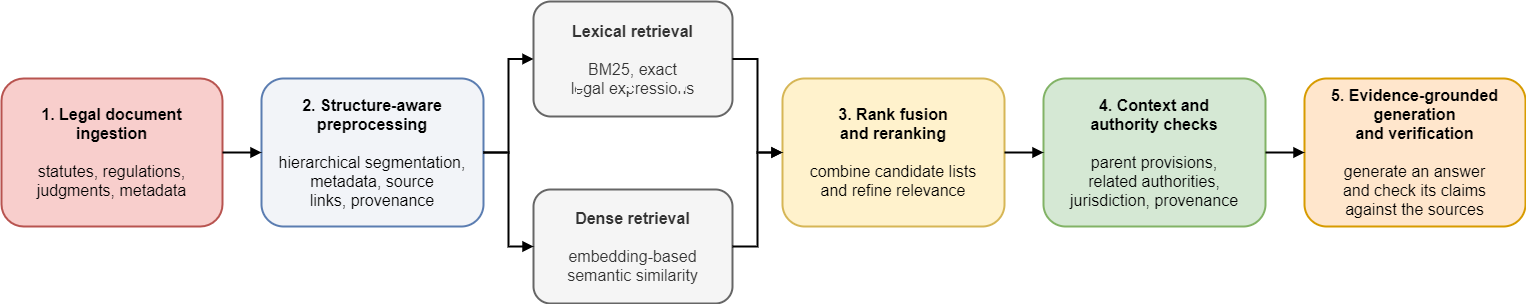
\includegraphics[width=\textwidth]{images/legal_rag_pipeline.png}
\caption{Conceptual architecture synthesizing complementary legal retrieval methods. This is a
proposed reference architecture, not a claim that every component has been validated together in a
single experiment.}
\label{fig:arch}
\end{figure*}


\subsection{Evaluating retrieval and RAG architectures}

We should assess a retrieval architecture independently of the quality of its generated answers.
The generator cannot reliably make up for evidence the retriever failed to return, and successful
retrieval does not establish that the generator interprets that evidence correctly.
Table~\ref{tab:metrics} summarizes the complementary metrics this requires, drawing on the
retrieval and evaluation literature this section discusses.

\begin{table*}[tp]
\centering
\caption{Complementary metrics for evaluating legal retrieval and RAG architectures.}
\label{tab:metrics}
\footnotesize
\setlength{\tabcolsep}{5pt}
\renewcommand{\arraystretch}{1.25}
\begin{tabularx}{\textwidth}{>{\raggedright\arraybackslash}p{4.0cm} >{\raggedright\arraybackslash}X >{\raggedright\arraybackslash}X}
\toprule
\textbf{Metric} & \textbf{What it measures} & \textbf{Why it matters in legal retrieval} \\
\midrule
Recall@$k$ / Precision@$k$ & Whether, and how purely, relevant evidence appears among the top $k$ results. & Finds needed authorities while bounding irrelevant material entering generation. \\
MRR / nDCG & How early a relevant result appears, and ranking quality under graded relevance. & Distinguishes highly relevant legal evidence from merely related passages. \\
Passage-level retrieval accuracy & Whether a system retrieved the specific supporting passage, not just the document \citep{pipitone2024}. & A correct document with the wrong passage still fails to support a generated answer. \\
Citation precision / recall & Proportion of citations that correctly support their claim, and of required support that is cited. & Measures whether references are evidentially useful and whether support is missing. \\
Unsupported-claim rate & Proportion of evaluated claims lacking adequate support in the permitted evidence. & Evaluates grounding beyond the mere presence of citations. \\
\bottomrule
\end{tabularx}
\end{table*}

These metrics need explicit annotation guidelines. Relevance can be graded at the document or
passage level with different results, and citation correctness needs a stated definition of what
counts as support. None of the architectural components this section discusses independently
guarantees legal correctness; their value depends on the corpus, provenance, and evaluation
protocol. The following year, 2025, is where the field put these retrieval techniques and evaluation
metrics to work in complete, deployed legal RAG systems, which Section~\ref{sec:maturing} takes up
next.

\section{Maturing Legal RAG Systems and Evaluation Research (2025)}
\label{sec:maturing}

Where 2024 established the problem of legal RAG and the metrics needed to evaluate it, 2025 is the
year complete systems and larger-scale evaluation studies arrived. This section follows eleven
studies from that year, organized into two groups: deployed or applied legal RAG systems, and the
evaluation, reliability, and survey literature that assessed them.

\subsection{Legal RAG applications}

\citet{buffa2025} published \textbf{JusBuild}, a system for drafting structured legal documents. It
segments existing documents into functional sections, retrieves relevant precedent sections during
drafting, and offers AI-generated suggestions while keeping a human professional in control of the
final formulation, shown in Figure~\ref{fig:jusbuild}. The authors evaluated JusBuild across datasets
that differ in language, template, and judicial matter. Its central design choice, keeping a human
in the loop rather than generating a final document on its own, reflects a judgment this survey
returns to directly in Section~\ref{sec:reliability}: retrieval-augmented drafting reduces, but does
not eliminate, the need for professional review.

% Figure reproduced from Buffa et al. (2025), "Enhancing legal document building with
% Retrieval-Augmented Generation" (Computer Law & Security Review), Fig. 1, for scholarly
% discussion and critique within this review. Copyright remains with the original
% authors/publisher.
\begin{figure*}[t]
\centering
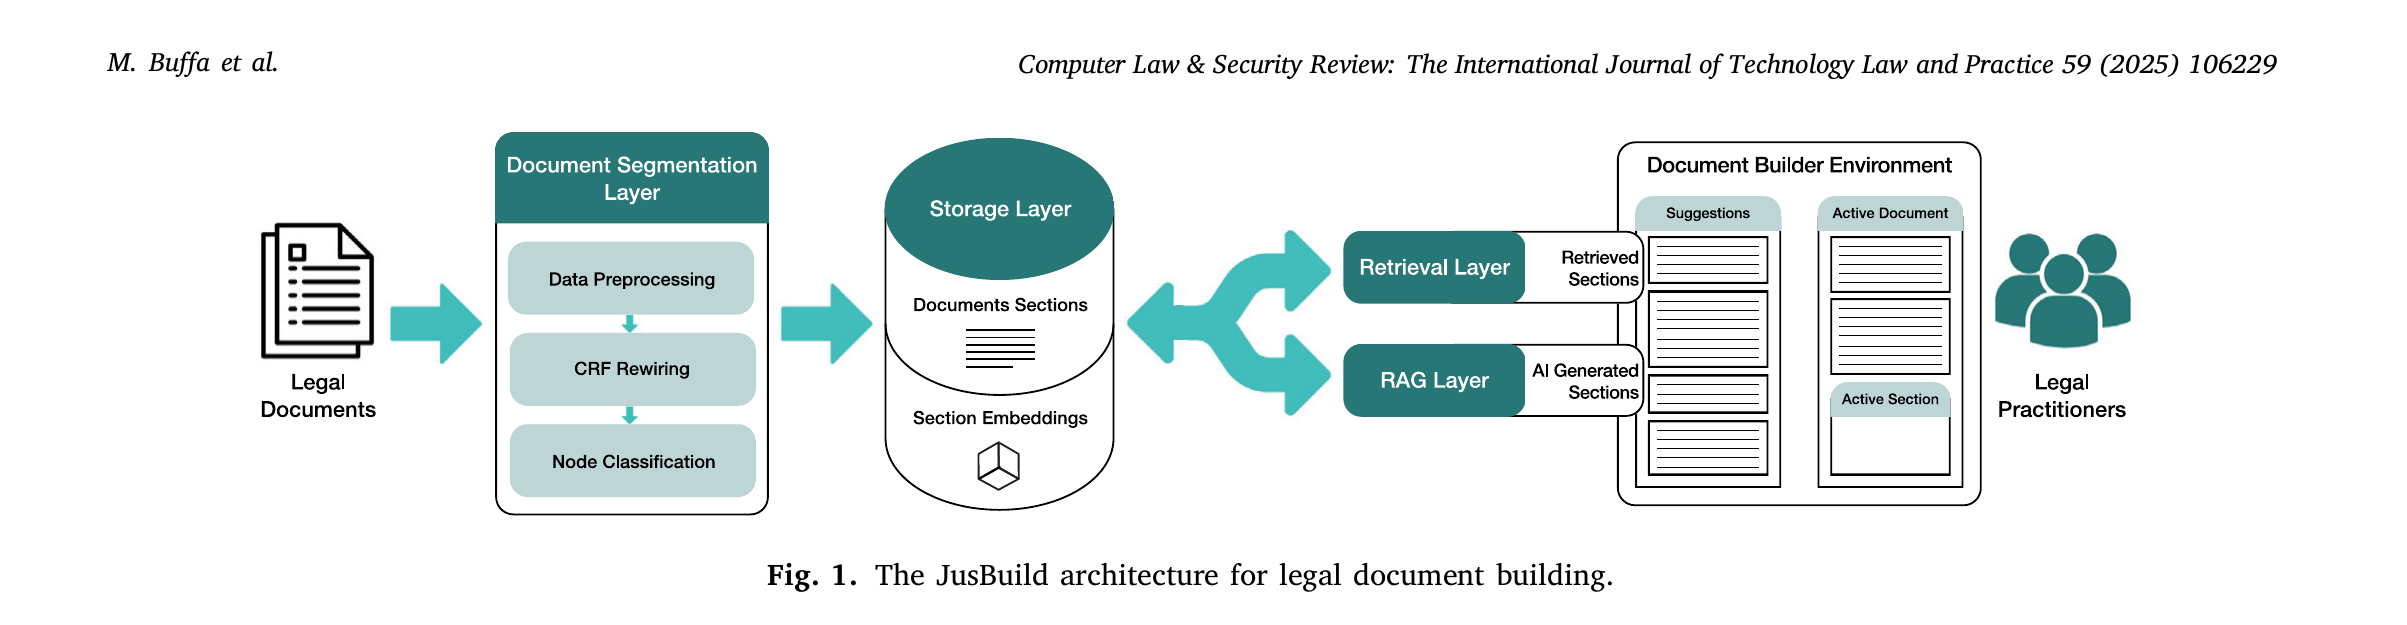
\includegraphics[width=\textwidth]{images/buffa2025_fig1.png}
\caption{Figure reproduced from \citet{buffa2025}: the JusBuild architecture for legal document
building. Legal documents pass through a Document Segmentation Layer (preprocessing, CRF
rewiring, node classification) into a Storage Layer of document sections and their embeddings.
At drafting time, a Retrieval Layer returns relevant retrieved sections and a RAG Layer returns
AI-generated sections, both surfaced to the legal practitioner inside the Document Builder
Environment alongside the document currently being drafted.}
\label{fig:jusbuild}
\end{figure*}


In the same year, \citet{zhang2025} proposed a multi-round RAG approach to comprehensive legal
document analysis. It retrieves evidence iteratively across several rounds instead of in a single
pass, which helps with questions no single retrieval step can resolve. \citet{ref312025} then
applied legal RAG to a jurisdiction this survey gives particular attention to: Pakistan. Their
framework combines semantic and keyword-based retrieval over selected Pakistani legal materials,
including the Code of Criminal Procedure and the Pakistan Penal Code. It shows concretely why
jurisdiction-specific evidence, not just a capable retrieval method, matters for legal question
answering. Section~\ref{sec:jurisdiction} examines this jurisdiction in depth, alongside the 2026
system that extends this line of work.

\subsection{Evaluation, reliability, and the surrounding survey literature}

The remaining 2025 studies turned attention from building legal RAG systems to assessing them, and
to surveying the field itself. \citet{premasiri2025} surveyed legal information extraction broadly.
They pulled together the extraction-focused line of work this survey traced from
\citet{chalkidis2017} in Section~\ref{sec:outcomes} through the knowledge-graph systems in
Section~\ref{sec:lm2023}. \citet{magesh2025} then directly tested the hallucination question
\citet{dahl2024} had raised the previous year. They assessed several leading commercial AI legal
research tools and found that hallucinations persisted despite those tools' use of
retrieval-augmented generation. This challenges any assumption that adding retrieval alone
guarantees a hallucination-free system. \citet{kelsall2025} carried out a rapid evidence review of
evaluation techniques for large language models in legal use cases. They found persistent gaps in
how researchers design and report legal AI evaluations. \citet{benedetto2025} proposed
\textbf{LR2}, a legal RAG system built specifically for legal reasoning over case law, and
\citet{italiani2025} looked at data generation and knowledge distillation as a way to improve legal
question answering without needing a full-scale retrieval pipeline for every deployment.
\citet{dugac2025} studied the harder problem of classifying legal \emph{interpretations} with large
language models. This is a more demanding task than classifying legal text by topic, because it
requires telling apart competing readings of the same provision. \citet{kim2025} stepped back from
individual systems to prioritize the challenges facing AI adoption in the legal domain more broadly.
They combined a systematic review with an expert-driven analytic hierarchy process. Finally,
\citet{tritto2025} surveyed causal artificial intelligence in legal language processing. They
pointed toward a research direction the systems discussed so far in this survey do not yet address:
reasoning about cause and effect instead of pattern similarity.

Read together, this year's studies show a field moving from asking whether legal RAG works in
principle to asking, with increasing precision, where specifically it fails and for whom. That
question motivates the final year of this survey's chronological account, 2026, where we situate
this survey's own comparative case study.

\section{Contemporary Systems and a Comparative Case Study (2026)}
\label{sec:2026}

This survey's chronological account reaches its final year, 2026, with the two systems this paper
also uses as a focused case study. Ten further studies, taken together, show how mature the field's
evaluation culture had become by the time this survey was written.

\subsection{Ren et al.\ and Legalyze: a comparative case study}

\citet{ren2026} and Legalyze \citep{hamza2026} both appeared in 2026, and both address legal RAG,
but they target different parts of the pipeline this survey has traced since
Section~\ref{sec:rag2024}. \citet{ren2026} concentrate on the training side. They synthesize
practice-question data from source law, then use that synthetic data together with RAG, an
LLM-based judge, and an Elo-ranking mechanism to improve a legal LLM's own generation. They evaluate
it on LawBench, a benchmark for Chinese legal language models. Legalyze \citep{hamza2026} instead
concentrates on the evidence side. It preserves statutory and judicial hierarchy through
structure-aware indexing, building directly on the structure-aware indexing described in
Section~\ref{sec:rag2024}. It combines lexical and dense retrieval through reciprocal-rank fusion,
the same technique \citet{cormack2009} introduced outside the legal domain in 2009. An agentic layer
then produces a citation-grounded answer over Pakistani legal materials, extending the
jurisdiction-specific work of \citet{ref312025} from the previous year. Figure~\ref{fig:legalyze-ren}
summarizes this contrast across research objective, dataset and jurisdiction, system architecture,
core contribution, and experimental evaluation.

\begin{figure*}[tp]
\centering
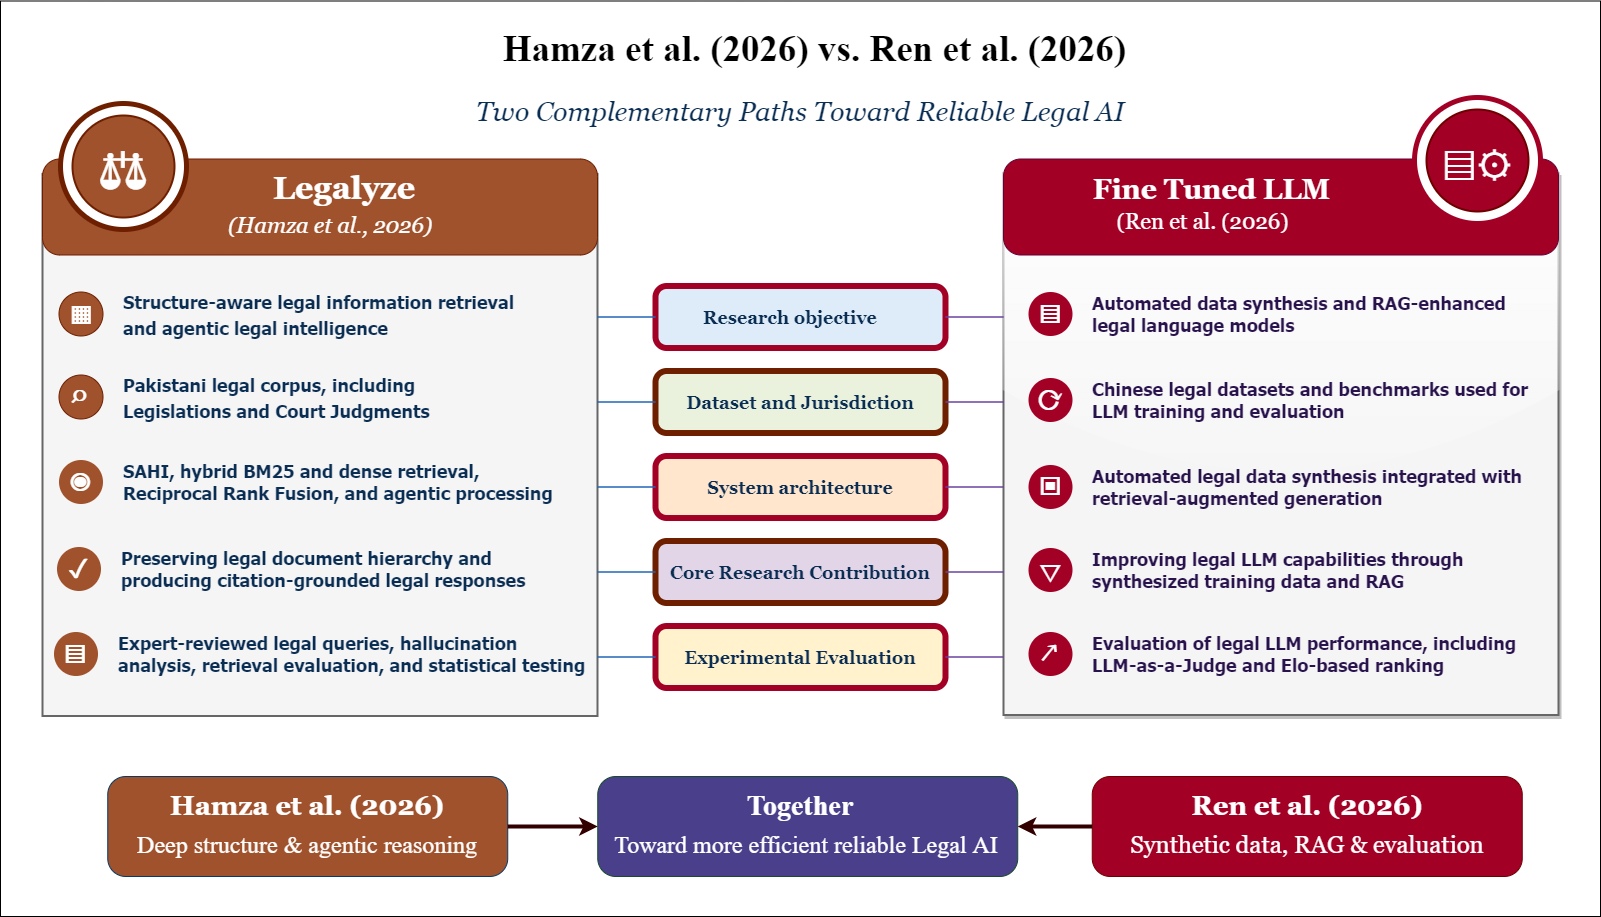
\includegraphics[width=\textwidth]{images/legalyze_vs_ren_2026_comparison.png}
\caption{Legalyze \citep{hamza2026} and the data-synthesis approach of \citet{ren2026} compared
across research objective, dataset and jurisdiction, system architecture, core research
contribution, and experimental evaluation. The two systems target different stages of the legal RAG
pipeline (evidence grounding versus training-data synthesis) and are best read as complementary
rather than directly competing.}
\label{fig:legalyze-ren}
\end{figure*}

The two approaches are complementary rather than competing. Data synthesis for training and
structure-aware retrieval for evidence grounding address different failure modes. A meaningful
head-to-head comparison would need a shared evaluation dataset, consistent query sets, and common
retrieval budgets, and none of these currently exist. Figure~\ref{fig:ren2026-arch} shows
\citeauthor{ren2026}'s own framework diagram, which makes this training-data-centric design
concrete. Data synthesis and Elo-ranking feed both a fine-tuned retrieval model and a
QLoRA-fine-tuned generation model, and together these form the Legal LLM Framework that answers a
user's query.

% Figure reproduced from Ren et al. (2026), "Automated data synthesis and
% retrieval-augmented generation for legal large language models" (Knowledge-Based
% Systems), Fig. 2, for scholarly discussion and critique within this review. Copyright
% remains with the original authors/publisher.
\begin{figure*}[t]
\centering
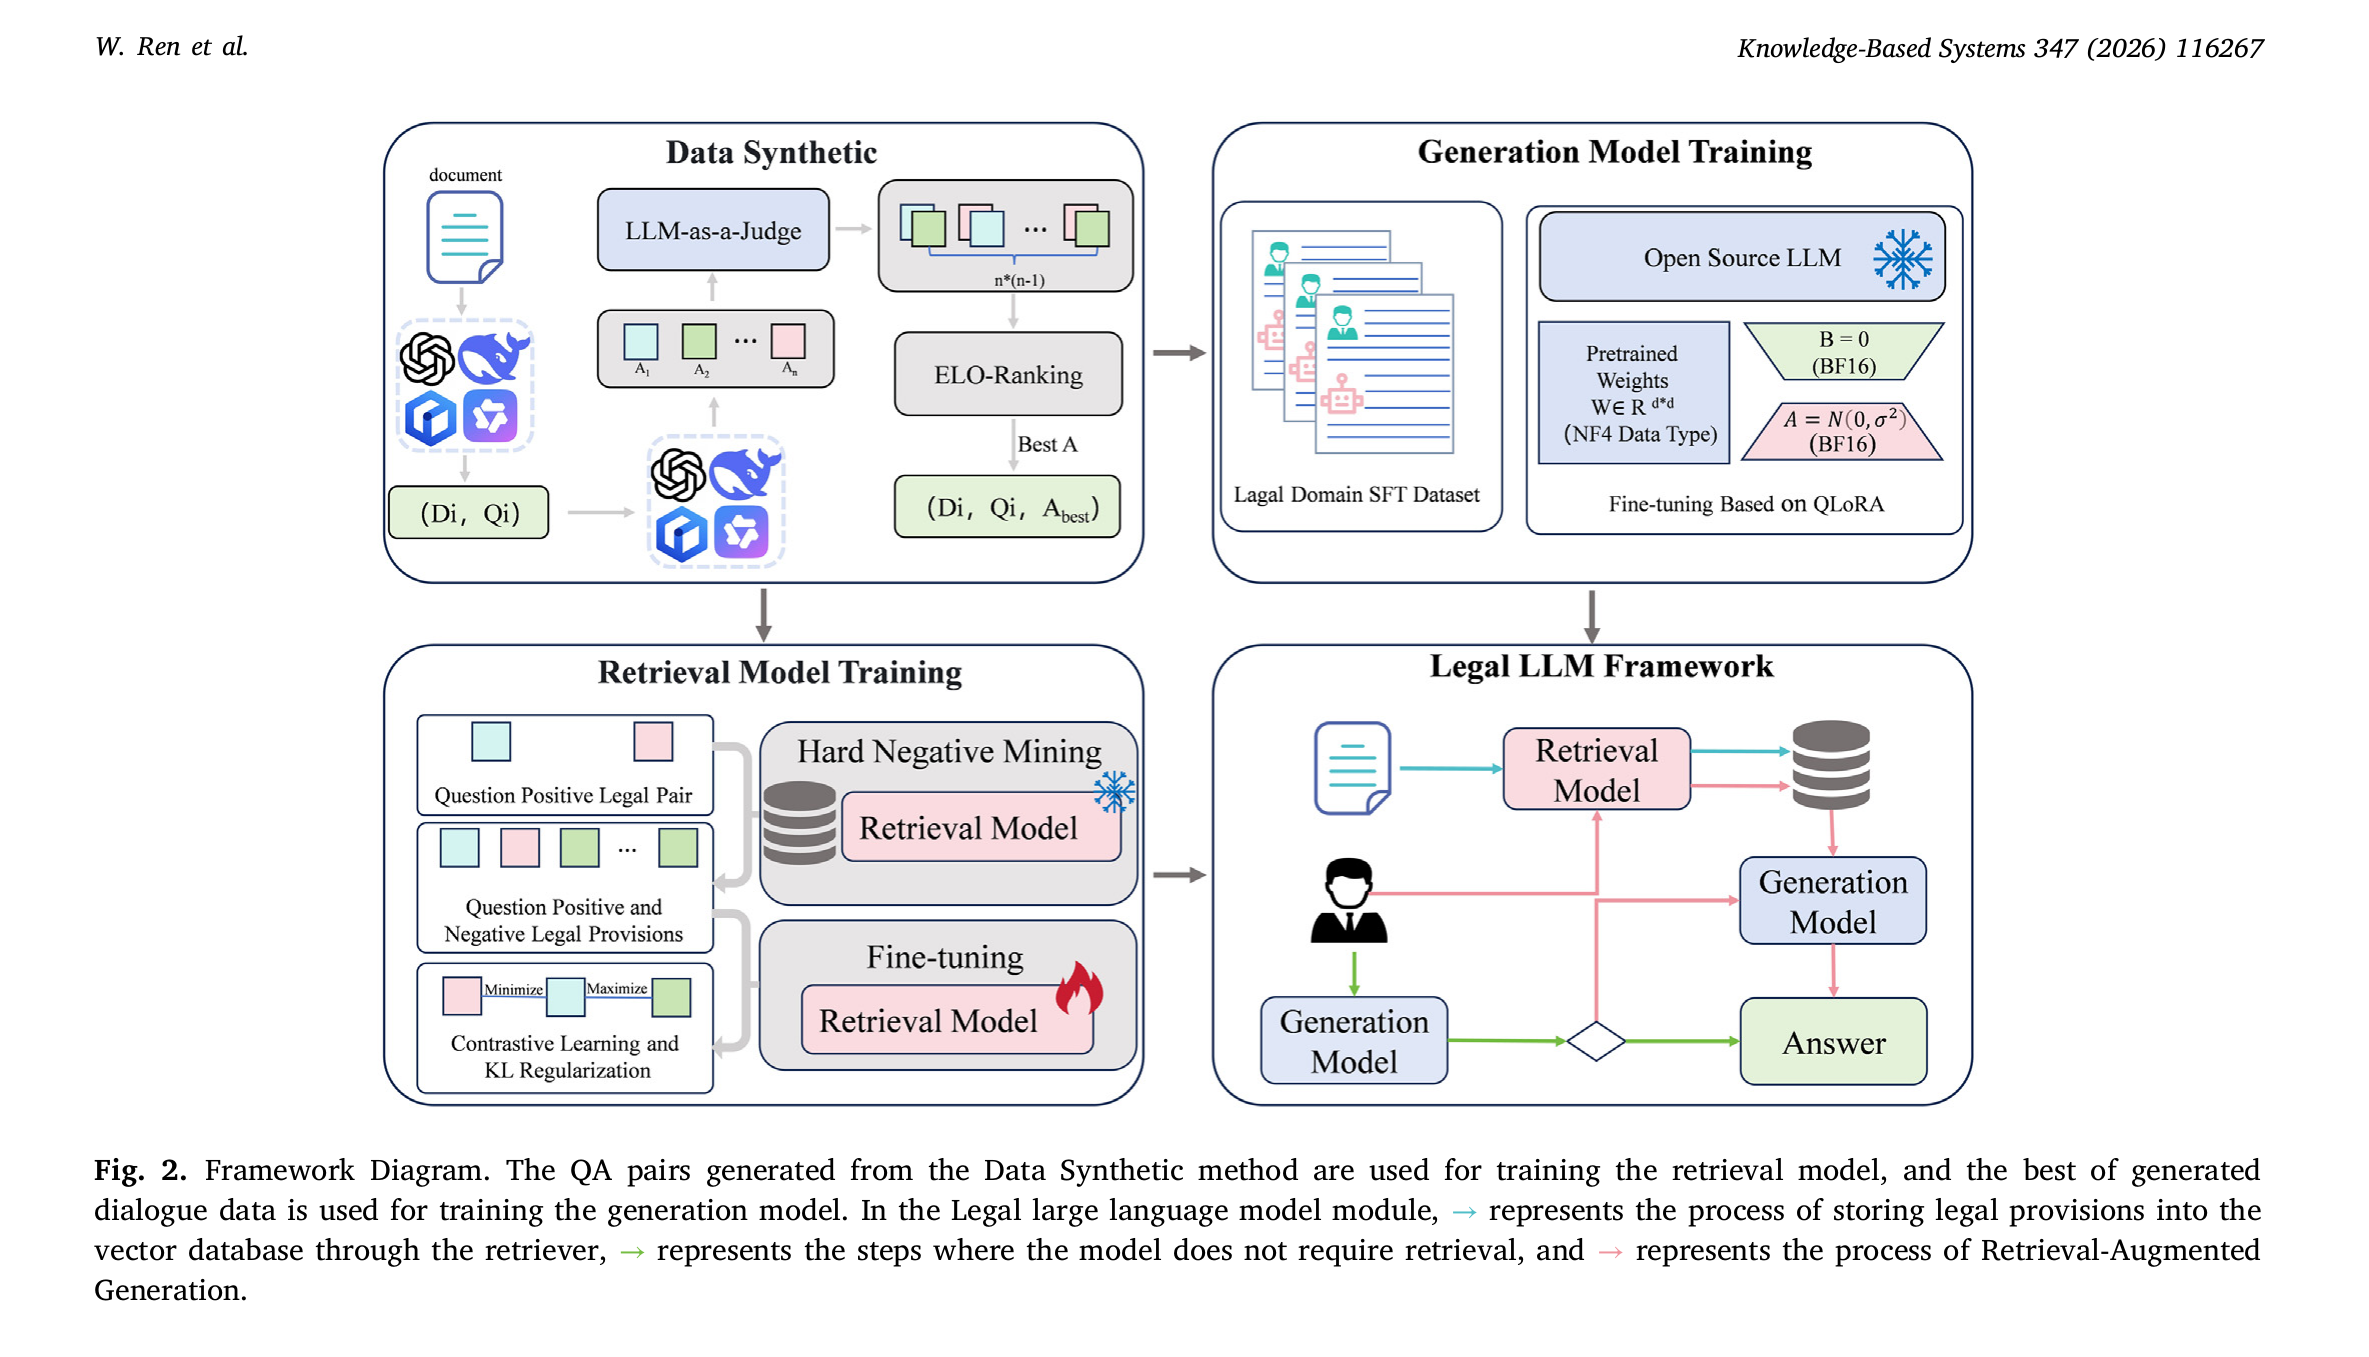
\includegraphics[width=\textwidth]{images/ren2026_fig2.png}
\caption{Figure reproduced from \citet{ren2026}: their framework diagram. QA pairs generated by
the Data Synthetic module (LLM-as-a-Judge selecting the best candidate answer via Elo-ranking)
train both the retrieval model, through hard-negative mining and contrastive fine-tuning, and the
generation model, through QLoRA fine-tuning of an open-source LLM on a legal-domain SFT dataset.
The resulting Legal LLM Framework routes a user's query through the fine-tuned retrieval model
and generation model to produce an answer, illustrating the training-data-centric design this
survey contrasts with Legalyze's evidence-centric design in Figure~\ref{fig:legalyze-ren}.}
\label{fig:ren2026-arch}
\end{figure*}


Table~\ref{tab:comp} places this pair alongside the other systems this survey has introduced
chronologically, now gathered in one place for direct comparison.

\begin{table*}[tp]
\centering
\caption{Comparison of representative legal AI systems discussed in this survey, in order of first appearance.}
\label{tab:comp}
\footnotesize
\setlength{\tabcolsep}{5pt}
\renewcommand{\arraystretch}{1.25}
\begin{tabularx}{\textwidth}{>{\raggedright\arraybackslash}p{2.6cm} >{\raggedright\arraybackslash}X >{\raggedright\arraybackslash}X >{\raggedright\arraybackslash}X}
\toprule
\textbf{System} & \textbf{Architecture and retrieval} & \textbf{Evidence verification} & \textbf{Key limitation} \\
\midrule
LEGAL-BERT \citep{chalkidis2020} & Legal-domain pretrained transformer; not inherently retrieval-based. & No inherent citation-verification mechanism. & Legal language competence does not establish evidence-grounded reasoning. \\
LexGLUE / LegalBench \citep{chalkidis2022, guha2023} & Standardized legal language and reasoning benchmarks. & Depends on the evaluated task and model. & Task scores do not directly measure citation support. \\
LegalBench-RAG \citep{pipitone2024} & Retrieval benchmark with annotated legal text segments. & Evaluates retrieval against annotated passages. & Does not, by itself, establish correctness of a generated answer. \\
JusBuild \citep{buffa2025} & Document segmentation with section-level vector retrieval for drafting. & Structured drafting workflow with human oversight. & Human review and drafting performance do not generalize to broader legal reliability. \\
Pakistani legal RAG \citep{ref312025} & Hybrid keyword and semantic retrieval over Pakistani statutes. & Grounded answering; verification assessed separately. & Grounding alone does not establish source completeness or claim-level entailment. \\
Ren et al.\ \citep{ren2026} & Synthetic data generation plus RAG for legal LLM training. & Supports the broader legal LLM pipeline. & Results depend on the selected benchmark (LawBench) and settings. \\
Legalyze \citep{hamza2026} & Hierarchical indexing, lexical and dense retrieval, reciprocal-rank fusion, agentic synthesis. & Citation-grounded response design over a hybrid retrieval pipeline. & Performance on one corpus and query set cannot establish universal correctness. \\
\bottomrule
\end{tabularx}
\end{table*}

The systems in Table~\ref{tab:comp} illustrate three design philosophies that emerged, in sequence,
across this survey's chronology. \textbf{Model-centric} approaches, LEGAL-BERT, LexGLUE, LegalBench,
adapt language models to legal text and reasoning patterns. \textbf{Retrieval-centric} approaches,
LegalBench-RAG and the Pakistani legal RAG framework, focus on locating relevant material.
\textbf{Structure-aware and workflow-oriented} approaches, JusBuild and Legalyze, also preserve
document organization. No single family addresses every legal AI problem, and evidence verification
remains distinct from retrieval in all three. That is exactly the problem
Section~\ref{sec:reliability} takes up as this survey's first synthesis chapter.

\subsection{Contemporary benchmarks, retrieval, and reasoning research}

Eight further studies from 2026 round out this survey's chronological account, each extending a
thread this survey has already introduced. \citet{yang2026} published a further survey of legal
case retrieval, extending the systematic account \citet{feng2024} gave in
Section~\ref{sec:rag2024} with two additional years of methods. \citet{goebel2026} summarized the
2025 edition of the COLIEE competition, continuing the series this survey has tracked since
\citet{goebel2023} and \citet{goebel2024}. \citet{butler2026} introduced \textbf{Legal RAG Bench},
the first full factorial evaluation of legal RAG that varies embedding models and generator LLMs
independently. They also proposed a hierarchical error-decomposition taxonomy that separates
hallucination, retrieval error, and reasoning error as distinct failure modes rather than folding
them into a single accuracy score. This taxonomy is central to how this survey discusses
reliability, so Figure~\ref{fig:rag-errors} in Section~\ref{sec:reliability} presents it in full.
\citet{chi2026} organized contemporary legal AI research around data, modelling, and evaluation,
and this survey's own methodology, in Section~\ref{sec:method}, used that broad landscape as
context for a narrower, chronological account. \citet{zhao2026} carried out a systematic review of
AI applications in litigation specifically, looking at challenges distinct from the
document-retrieval and drafting focus of most systems discussed so far. \citet{afane2026}
benchmarked legal RAG specifically on statutory surveys, testing the promise and limits of
AI-generated summaries of legislative text across jurisdictions. \citet{silva2026} evaluated RAG
systems in Brazilian civil procedure and reported a finding that echoes a theme recurring throughout
this survey since Section~\ref{sec:rag2024}: semantic similarity is not legal correctness, and a
retrieved passage that resembles the query in meaning can still fail to establish the legal point at
issue. Finally, \citet{le2026} proposed a three-tier knowledge-graph RAG architecture for legal
question answering, extending the graph-based retrieval line of work this survey has followed from
\citet{sovrano2020} in 2020, through \citet{zhu2022} in 2022, into a retrieval architecture with
three explicit levels of graph abstraction.

The chronological account is now complete, running from \citet{ashley1991} in 1991 to this final
group of 2026 studies. The rest of this survey turns from narrating the field's history to
synthesizing what it has established. Section~\ref{sec:reliability} draws together everything this
survey has said about hallucination, citation verification, and the Legal RAG Bench taxonomy just
introduced. Section~\ref{sec:jurisdiction} draws together its jurisdiction- and language-specific
findings. Section~\ref{sec:future} sets out the research agenda that follows from the complete
chronology.

\section{Synthesis: Reliability, Hallucination, and Legal Citation Verification}
\label{sec:reliability}

The chronological account in Sections~\ref{sec:foundations}--\ref{sec:2026} raised the reliability
problem repeatedly without resolving it. \citet{dahl2024} documented fabricated authorities in 2024.
\citet{magesh2025} found hallucinations persisting in commercial legal research tools despite their
use of RAG in 2025. \citet{butler2026} proposed a formal taxonomy for telling different kinds of
failure apart in 2026. This section draws those threads together into a single account of what legal
AI reliability actually requires.

Access to external evidence does not automatically make a legal answer reliable. A system may
retrieve a relevant document but misread its meaning, miss an exception, cite the wrong passage, or
draw a conclusion the retrieved evidence does not support. Legal correctness depends on more than
textual similarity. An answer can accurately reproduce a sentence from a judgment while still
misrepresenting its holding. It can identify the correct statute while missing an amendment or
jurisdictional restriction that affects its application. We can organize reliability around three
related questions, and none of them can stand in for the others. Did the system retrieve the right
evidence? Does the evidence support the claim, rather than merely discuss a similar topic? Does the
claim apply legally, given the jurisdiction, date, and procedural context?

\citet{butler2026} gave this last distinction a precise, testable form. Instead of reporting one
aggregate accuracy score, their hierarchical error-decomposition taxonomy, reproduced in
Figure~\ref{fig:rag-errors}, separates three failure modes. It uses three binary signals the authors
collected per question, embedding model, and LLM.

% Figure reproduced from Butler and Butler (2026), "Legal RAG Bench: An End-to-End
% Benchmark for Legal RAG", Figure 1, for scholarly discussion and critique within this
% review. Copyright remains with the original authors/publisher.
\begin{figure*}[t]
\centering
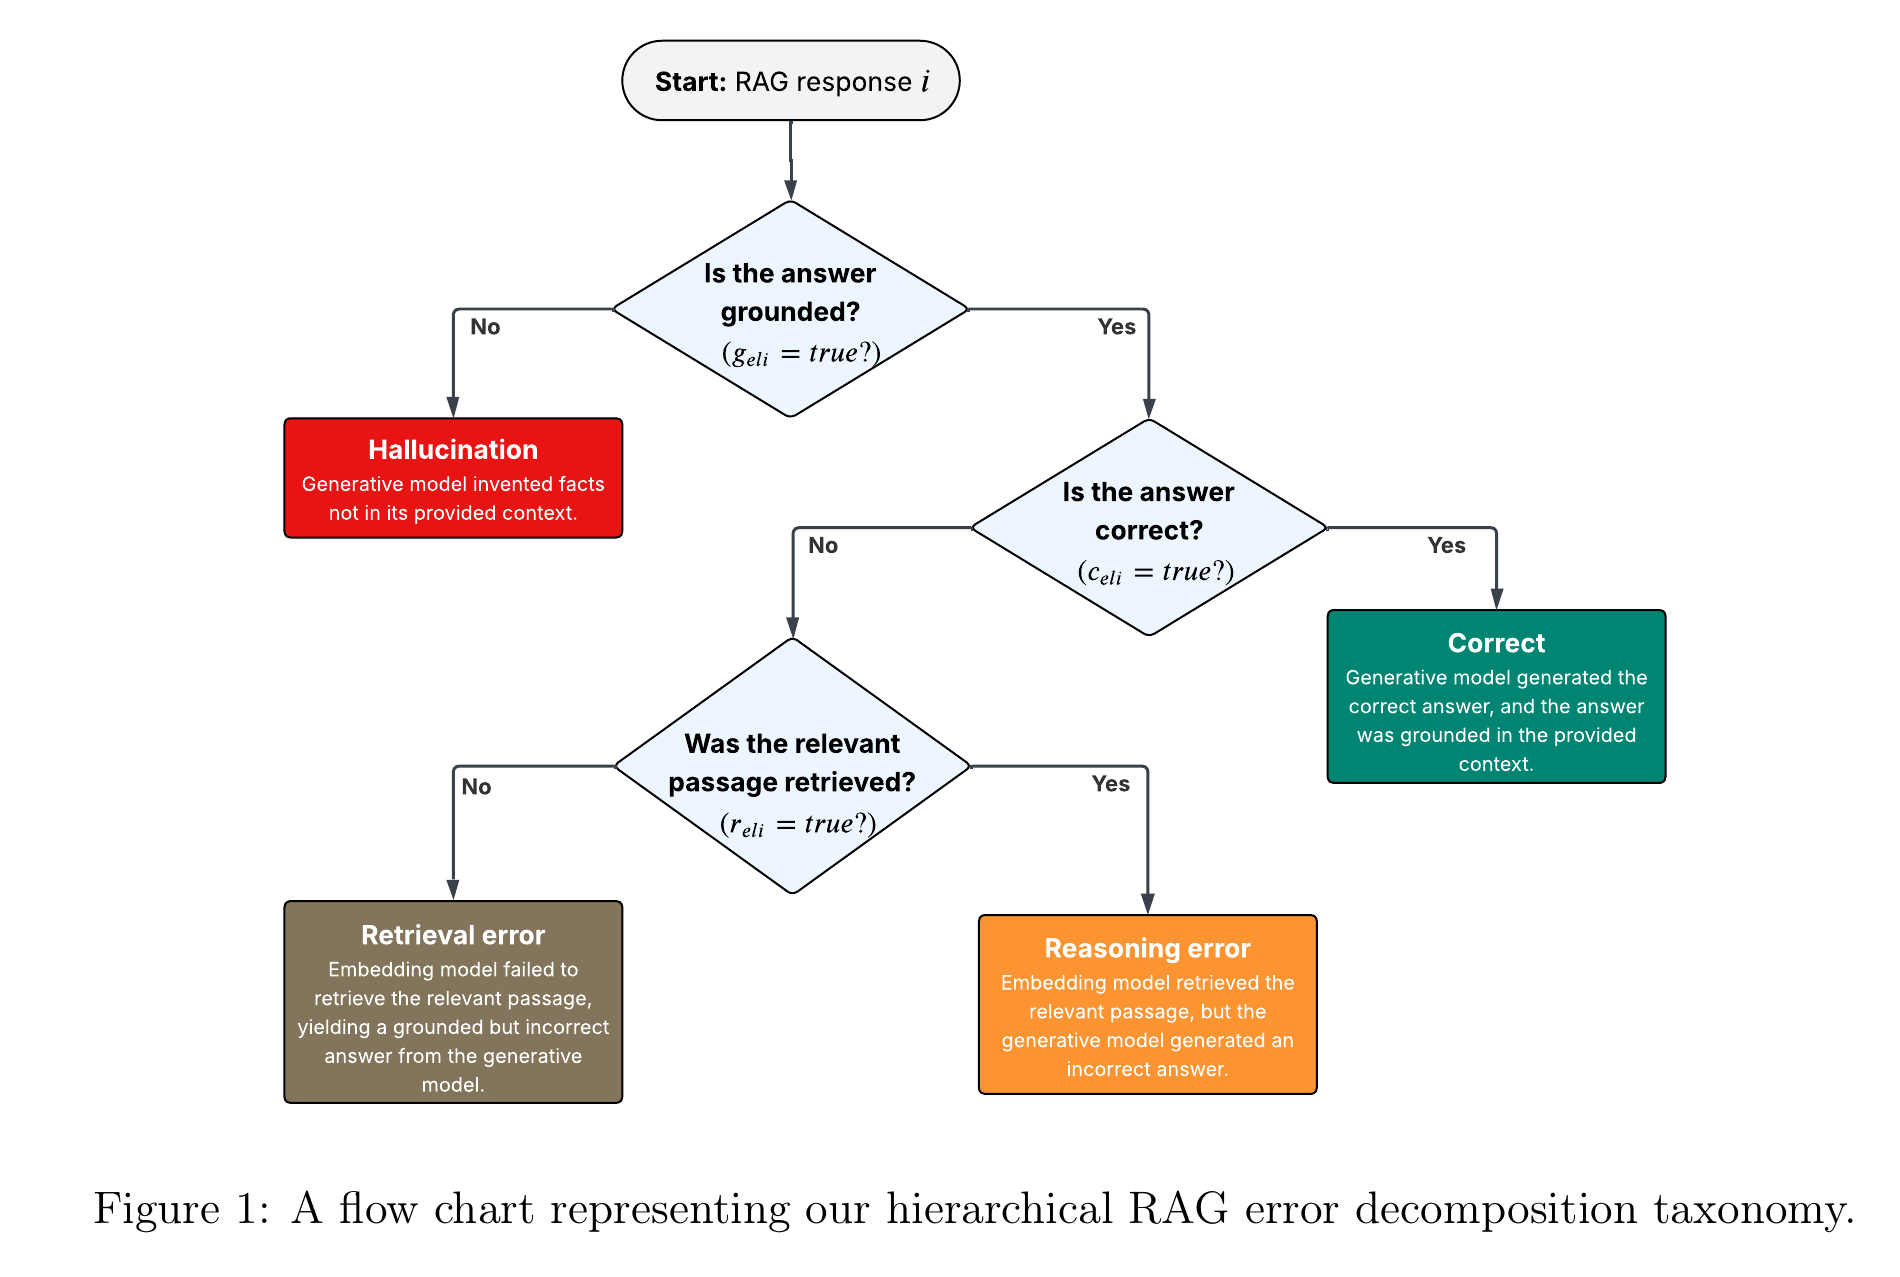
\includegraphics[width=\textwidth]{images/butler2026_fig1.png}
\caption{Figure reproduced from \citet{butler2026}: the hierarchical RAG error-decomposition
taxonomy. Rather than reporting one aggregate accuracy score, the taxonomy separates three
distinct failure modes using three binary signals collected per question, embedding model, and
LLM: groundedness ($g$, whether the answer is supported by what was retrieved), retrieval
accuracy ($r$, whether the annotated supporting passage was actually retrieved), and correctness
($c$, whether the answer entails the reference answer). This distinguishes an ungrounded
hallucination from a grounded answer that is wrong because retrieval failed, and from a grounded,
correctly retrieved answer that the generator still reasoned about incorrectly.}
\label{fig:rag-errors}
\end{figure*}


An ungrounded \textbf{hallucination}, where what the system retrieved does not support the answer,
differs from a grounded answer that is wrong because the system never retrieved the needed passage,
a \textbf{retrieval error}. Both differ again from a grounded, correctly retrieved answer that the
generator still reasoned about incorrectly, a \textbf{reasoning error}. This distinction matters in
practice, because it determines what fixing the system actually requires. A hallucination calls for
stronger grounding and abstention. A retrieval error calls for a better retriever or a richer index.
A reasoning error calls for improving how the generator uses the evidence it already has.
Table~\ref{tab:failures} extends this taxonomy with the broader set of reliability failures this
survey has encountered across its chronology.

\begin{table*}[tp]
\centering
\caption{Reliability failure modes in legal AI and possible mitigations.}
\label{tab:failures}
\footnotesize
\setlength{\tabcolsep}{5pt}
\renewcommand{\arraystretch}{1.25}
\begin{tabularx}{\textwidth}{>{\raggedright\arraybackslash}p{2.6cm} >{\raggedright\arraybackslash}X >{\raggedright\arraybackslash}X}
\toprule
\textbf{Failure type} & \textbf{Description} & \textbf{Possible mitigation} \\
\midrule
Hallucination \citep{dahl2024, butler2026} & The system invents a case, statute, or citation, or asserts a claim the retrieved evidence does not support. & Citation resolution against authoritative databases; abstention when evidence is missing. \\
Retrieval error \citep{butler2026} & The answer is grounded in retrieved text, but the system never retrieved the passage it actually needed. & A better retriever, hybrid retrieval, or a richer structure-aware index. \\
Reasoning error \citep{butler2026} & The system retrieved the correct passage, but the generator still drew an incorrect conclusion from it. & Claim-to-passage entailment checking and role-aware judgment analysis. \\
Incomplete evidence & The system retrieved a relevant exception, counter-authority, or condition only partially. & Query expansion and retrieval of related provisions. \\
Outdated or jurisdictionally mismatched law & The system applies a superseded or foreign authority, as the Pakistani case study in Section~\ref{sec:jurisdiction} illustrates. & Effective-date metadata and jurisdiction filtering. \\
\bottomrule
\end{tabularx}
\end{table*}

We should not treat a citation as reliable merely because it resolves to an existing document.
Verification splits into four checks. Citation resolution asks whether the cited authority exists
and whether a reader can locate it. Passage verification asks whether the cited passage actually
contains the relevant language. Claim-support verification asks whether the passage actually
supports the claim. Applicability verification asks whether the authority applies to the
jurisdiction, date, and procedural context of the question. This means verification should work at
the level of individual claims, not a whole response, since a long answer can contain several
supported statements and one unsupported conclusion that a document-level check would miss.
\citet{pipitone2024}'s focus on retrieving precise text segments, introduced in
Section~\ref{sec:rag2024}, reinforces the importance of granular evidence. Precise retrieval and
legal entailment still remain separate requirements, though: finding the correct passage does not by
itself show that the generated interpretation of it is valid. We should not read either
\citet{dahl2024} or \citet{magesh2025} as establishing one universal hallucination rate. Results
depend on the tools, tasks, jurisdictions, and definitions of error each evaluation uses. That is
why a reproducible evaluation should disclose the corpus's jurisdiction and temporal scope, the
source of its test questions, the operational definition of hallucination it uses, and the
annotation protocol and reviewer expertise behind its results, in the spirit of the groundedness,
retrieval-accuracy, and correctness signals \citet{butler2026} report separately instead of folding
into one number.

Multiple safeguards handle reliability better than any single verification component. These
include authoritative source management that records provenance, jurisdiction, and effective dates.
They include retrieval and ranking across the lexical, dense, and structure-aware methods described
in Section~\ref{sec:rag2024}. They include claim-level generation that ties each material assertion
to a supporting passage. They include verification that resolves citations and tests claim support.
And they include a qualified response or abstention when evidence is missing or contradictory. We
put this conceptual workflow together for this survey; it is not a claim that every reviewed system
implements all five stages. Agentic architectures, such as the one Legalyze uses in
Section~\ref{sec:2026}, can coordinate these safeguards, but adding agents does not automatically
improve correctness. If the agents share the same incomplete corpus, or repeat the same unsupported
assumption, orchestration can reproduce the underlying error instead of correcting it. The central
lesson of this chapter, and arguably of this entire survey, is that legal AI reliability demands an
evidence-to-claim evaluation. A dependable system must retrieve appropriate authority, keep its
context, generate claims that follow from the evidence, verify citations, and recognize when legal
applicability remains uncertain.

\section{Synthesis: Jurisdiction, Document Structure, and Multilingual Legal AI}
\label{sec:jurisdiction}

This chapter draws together a theme this survey has touched at several points along its chronology,
most directly through \citet{ref312025} and Legalyze \citep{hamza2026} in Section~\ref{sec:2026}:
legal information retrieval is jurisdiction-dependent in a way general-purpose retrieval is not. The
relevance of a document depends not only on its topic but on its legal authority, jurisdiction,
temporal validity, and relationship to the question asked. A question on Pakistani criminal
procedure should prioritize applicable Pakistani legislation and judicial decisions. A semantically
similar provision from another jurisdiction may help explain a general concept, but a system should
not automatically treat it as governing authority. Jurisdiction-sensitive retrieval therefore has to
consider territorial and institutional jurisdiction, authority type (legislation, binding judgment,
persuasive judgment, commentary), temporal validity, procedural context, and precedential
relationships. An embedding model, of the kind described in Section~\ref{sec:rag2024}, can mark two
passages as highly similar without determining whether either is legally applicable. These
constraints should shape retrieval and verification directly, not just appear as explanatory text in
the final answer.

Legal documents also carry multiple layers of organization. Statutes divide into parts, sections,
subsections, and provisos. Judgments contain procedural history, issues, reasoning, and final
orders. Fixed-size chunking can separate a provision from its heading, definition, or exception,
producing a fragment that remains readable while losing the context legal interpretation needs. The
structure-aware retrieval techniques described in Section~\ref{sec:rag2024} address this in four
ways. Hierarchical metadata links each passage to its document, chapter, and section.
Context-preserving chunking keeps headings and exceptions attached. Parent-child retrieval recovers
a passage's broader context on demand. Provenance preservation records the source document and
version a reader needs to verify it. Pakistan shows why this matters in practice. Its legal
information needs span the Constitution, the Pakistan Penal Code, the Code of Criminal Procedure,
the Qanun-e-Shahadat Order, and judicial decisions that serve different legal functions, so a corpus
can be large and still miss relevant amendments or authoritative judgments. A provision's wording or
interpretation can also change over time. A system has to track this by recording source dates and
applicable versions, instead of assuming the newest document is the most authoritative.
\citet{ref312025} demonstrated a RAG-based framework combining semantic and keyword retrieval over
selected Pakistani legal materials. Legalyze \citep{hamza2026} extended this with hierarchical
indexing, hybrid retrieval, and rank fusion, as Section~\ref{sec:2026} described. A meaningful
comparison between the two would still need a shared evaluation dataset, consistent query sets, and
common retrieval and answer-quality measures.

A further challenge arises when a user's query language differs from the language or script of the
authoritative source. This is common when Pakistani legal questions appear in Urdu or Roman Urdu
while the relevant statute or judgment appears in English. Direct translation alone can fall short,
because legal concepts carry jurisdiction-specific meanings that do not map exactly across
languages. Table~\ref{tab:multilingual} summarizes the main technical approaches.

\begin{table*}[t]
\centering
\caption{Technical approaches to multilingual legal retrieval.}
\label{tab:multilingual}
\footnotesize
\setlength{\tabcolsep}{5pt}
\renewcommand{\arraystretch}{1.25}
\begin{tabularx}{\textwidth}{>{\raggedright\arraybackslash}p{3.0cm} >{\raggedright\arraybackslash}X >{\raggedright\arraybackslash}X}
\toprule
\textbf{Approach} & \textbf{Main advantage} & \textbf{Main limitation} \\
\midrule
Query translation & Enables use of existing monolingual retrieval infrastructure. & Translation may distort legal terms or procedural meaning. \\
Multilingual dense retrieval & Supports cross-language semantic matching in a shared embedding space. & Similar embeddings do not guarantee legal-concept equivalence. \\
Transliteration normalization & Helps retrieve Roman Urdu and Urdu spelling variants. & Many transliterations remain ambiguous or inconsistent. \\
Legal terminology alignment & Links expressions to jurisdiction-specific legal concepts. & Requires curated terminology and entity-linking resources. \\
\bottomrule
\end{tabularx}
\end{table*}

A practical architecture combines these methods instead of relying on just one. Language
identification and transliteration normalization process the query first. Legal entity linking and
terminology alignment then identify the relevant statutes and concepts. Retrieval searches both the
original and normalized query before rank fusion and jurisdictional filtering. The system should
keep the original query and the original authoritative passage throughout. Translation can support
retrieval, but the final answer should not quietly substitute a translated interpretation for the
governing source text. We should also carry out evaluation separately for each supported language,
rather than assume it carries over from an English-only benchmark. Jurisdiction, document structure,
and language are consequently tied together, not separable concerns. Language normalization can help
locate a relevant provision, but document structure still has to preserve its context. Hierarchical
indexing can identify the correct section, but jurisdictional and temporal checks remain necessary
to work out whether it actually applies. For Pakistani legal AI, the resulting requirement is clear:
effective retrieval needs more than semantic similarity. It needs legal hierarchy, authority
relationships, temporal metadata, source provenance, and cross-language concept alignment, all
working together. That requirement leads into the open research directions we discuss next.

\section{Open Challenges and Future Research Directions}
\label{sec:future}

Contemporary legal AI, as the chronological account in Sections~\ref{sec:foundations}--\ref{sec:2026}
has shown, has made genuine progress in legal language understanding, evidence retrieval, document
drafting, and agentic processing. These capabilities, though, remain difficult to bring together
into a system that consistently returns relevant, applicable, and verifiable legal answers. The
central research challenge is therefore not to produce more fluent legal text, but to build systems
that retrieve authoritative evidence, preserve its legal context, reason over relationships between
sources, and verify the claims they generate. Seven directions follow from the synthesis in
Sections~\ref{sec:reliability} and~\ref{sec:jurisdiction}.

\textbf{Knowledge-graph-grounded retrieval.} Flat indexes struggle with questions that need
relationships across documents, such as connecting a provision to its definition and to the
judgments that interpret it. Future work should combine graph-based and text retrieval. It should
keep provenance for every relationship and tell apart explicitly stated facts from inferred
connections. Researchers could evaluate this by comparing a text-only baseline, a graph-only
method, and a combined architecture on multi-hop legal questions.

\textbf{Multilingual and low-resource retrieval.} Researchers should evaluate cross-lingual
retrieval models, terminology alignment, and transliteration-aware indexing in two ways: by
measuring how retrieval performance varies across English, Urdu, and Roman Urdu queries, and by
checking whether legal entity linking reduces errors involving statutory names and section numbers.
The central risk here is mistaking linguistic similarity for legal equivalence.

\textbf{Structure-aware indexing.} Researchers should compare fixed-size, semantic, and hierarchical
chunking under the same conditions. They should pay particular attention to whether preserving
structure improves downstream answer quality beyond its effect on retrieval recall. Parsing
failures also deserve attention: malformed PDFs, inconsistent numbering, and broken cross-references
can all propagate errors through the rest of the pipeline.

\textbf{Claim-level evidence verification.} Citation-grounded generation is not enough if a system
only checks whether a response contains references. Future architectures should tie each material
claim to the specific passage meant to support it. They should resolve citations and flag
unsupported or contradictory statements, because legal support is often more complex than ordinary
textual entailment: a passage may state a general rule while a different passage supplies the
exception.

\textbf{Agentic legal AI with explicit quality gates.} Orchestration should focus on
evidence-controlled workflows rather than simply adding more agents. Each stage needs explicit input
requirements, output contracts, and quality checks. Experiments should compare single-agent and
multi-agent alternatives under equivalent retrieval settings. Without such controls, we cannot
reliably credit improvements to agentic orchestration.

\textbf{Temporal and authority-aware reasoning.} Statutes get amended, and judgments get
distinguished or overruled, over time. Future systems should therefore represent effective dates and
relationships between authorities. They should not assume the newest document is necessarily the
most applicable.

\textbf{Reproducible evaluation and realistic benchmarks.} Future benchmarks should combine
retrieval and generation evaluation while keeping separate scores for each stage, following the
groundedness, retrieval-accuracy, and correctness decomposition this survey described in
Section~\ref{sec:reliability}. They should include difficult cases involving exceptions and
competing authorities. They should also report dataset construction, annotation instructions, and
inter-annotator agreement, so researchers can tell genuine architectural improvements apart from
differences in test construction.

Table~\ref{tab:agenda} pulls these directions together into measurable research objectives.

\begin{table*}[tp]
\centering
\caption{Open challenges and measurable research objectives.}
\label{tab:agenda}
\footnotesize
\setlength{\tabcolsep}{5pt}
\renewcommand{\arraystretch}{1.25}
\begin{tabularx}{\textwidth}{>{\raggedright\arraybackslash}p{3.6cm} >{\raggedright\arraybackslash}X >{\raggedright\arraybackslash}X}
\toprule
\textbf{Research challenge} & \textbf{Proposed direction} & \textbf{Example evaluation} \\
\midrule
Missing cross-document relationships & Combine knowledge graphs with text retrieval. & Recall on multi-hop questions and graph-relation accuracy. \\
Low-resource multilingual queries & Multilingual retrieval with terminology alignment. & Language-specific Recall@$k$ and expert-assessed correctness. \\
Loss of legal hierarchy & Structure-aware indexing and parent-child retrieval. & Structural extraction accuracy and downstream answer quality. \\
Unsupported legal claims & Claim-level evidence verification. & Claim-support precision, recall, and unsupported-claim rate. \\
Unreliable agentic workflows & Modular orchestration with explicit quality gates. & Correctness, failure recovery, latency, and ablation results. \\
Outdated or inapplicable authorities & Temporal and authority-aware retrieval. & Outdated-law error rate and applicability accuracy. \\
Incomparable research results & Shared benchmarks and reproducible protocols. & Cross-system results under common data and evaluation rules. \\
\bottomrule
\end{tabularx}
\end{table*}

These directions depend on one another. Knowledge graphs support authority-aware retrieval only if
source extraction is accurate. Multilingual retrieval improves access but still needs jurisdictional
filtering. Structure-aware indexing preserves context that claim-level verification can then assess.
Agentic workflows can coordinate all of this, but only reproducible evaluation can show whether the
resulting system is actually more dependable. The most promising agenda is therefore an integrated
one: knowledge-graph-grounded, multilingual, structure-aware legal retrieval with explicit evidence
verification and reproducible evaluation. This agenda carries into the next decade the same two
questions this survey opened with in 1991: how should we represent legal knowledge, and how should
we trust a system's reasoning over it?

\section{Conclusion}
\label{sec:conclusion}

This survey has told one continuous story, in the order it actually happened. It runs from Ashley's
HYPO in 1991, through case-based reasoning's reframing as lazy learning in 2003, through the
statistical and neural prediction of legal outcomes between 2014 and 2018, through domain-adapted
legal language models and their benchmarks between 2020 and 2023, through the emergence of legal
retrieval-augmented generation in 2024, through a year of maturing systems and sharper evaluation in
2025, and on to the contemporary systems of 2026, Legalyze among them. If we read the field this
way, instead of organizing it by topic, a specific pattern becomes visible, one a topic-first
account can obscure: each stage responded to a concrete limitation of the one before it. Case-based
reasoning showed that legal relevance depends on more than textual similarity, but it struggled to
scale. Quantitative outcome prediction scaled, but could not explain its own reasoning. Legal
language models processed text fluently, but could not guarantee they were right.
Retrieval-augmented generation connected generation to external evidence, but retrieval quality,
legal correctness, and citation support turned out to be three separate problems, not one.

The comparative case study of Legalyze and Ren et al.\ (2026) shows this same pattern at the scale
of a single year. Two systems appeared in the same year, addressed the same general problem, and
chose to solve different halves of it. One used structure-aware evidence grounding; the other used
synthetic training data. Neither choice is complete on its own. That is exactly the lesson this
survey's reliability synthesis drew from \citet{butler2026}'s error taxonomy: a hallucination, a
retrieval error, and a reasoning error call for three different fixes, and a system that only
addresses one of them will still fail on the other two. The jurisdiction and multilingual synthesis
extends this lesson geographically. In contexts such as Pakistan, effective systems have to connect
user queries, which users may express in English, Urdu, or Roman Urdu, to the appropriate legal
sources while preserving statutory hierarchy, judicial context, and provenance. A system that
researchers validate only on English-language, single-jurisdiction data has not yet shown that it
generalizes.

Future research should prioritize structure-preserving retrieval, provenance-aware legal knowledge
graphs, multilingual query processing, claim-level citation verification, and agentic workflows with
explicit quality gates. Researchers should test these through reproducible benchmarks that cover the
complete evidence-to-answer pipeline and report retrieval effectiveness, legal correctness, citation
support, and cost, without collapsing them into a single score, in the spirit of the groundedness,
retrieval-accuracy, and correctness decomposition this survey has described. The goal of legal AI
should not be to replace legal judgment with fluent automated responses. It should be to make legal
information more accessible, systematic, and auditable, while keeping the distinction between
retrieved evidence, model-generated interpretation, and conclusions that need professional review.
Thirty-five years after Ashley first asked whether a computer could compare legal cases, the field's
next stage will depend less on generation alone and more on the ability to retrieve, contextualize,
verify, and reproduce evidence-supported legal reasoning.


\section*{Declaration of Generative AI and AI-assisted Technologies in the Writing Process}
The authors used AI for linguistic purposes only, and not for idea generation or creation.

\bibliographystyle{plainnat}
\bibliography{references}

\FloatBarrier
\end{document}
